\section*{California Case Study}

\subsection*{Background}

The state of California is geographically large and diverse in demography and land use. Per 2022 US census bureau annual estimates [SOURCE], California's population numbers over 39 million persons with around 32.5 million living in 482 Incorporated Places including cities and towns. These Places range from Los Angeles with a population of 3.8 million located near the coast to Amador City with a population of 201 located in the Sierra foothills. Connecting these disparate locations are a collection of major road transit corridors. Running roughly north-south are S-1/101, I-5/S-99, and U-395. Running roughly east-west are I-8, I-10, I-15, I-40, and I-80. Much of the traffic on the east-west corridors represents interactions with adjoining states. Incorporated Places in California are shown in Figure \ref{fig:california_incorporated_places}.

\begin{figure}[H]
	\centering
	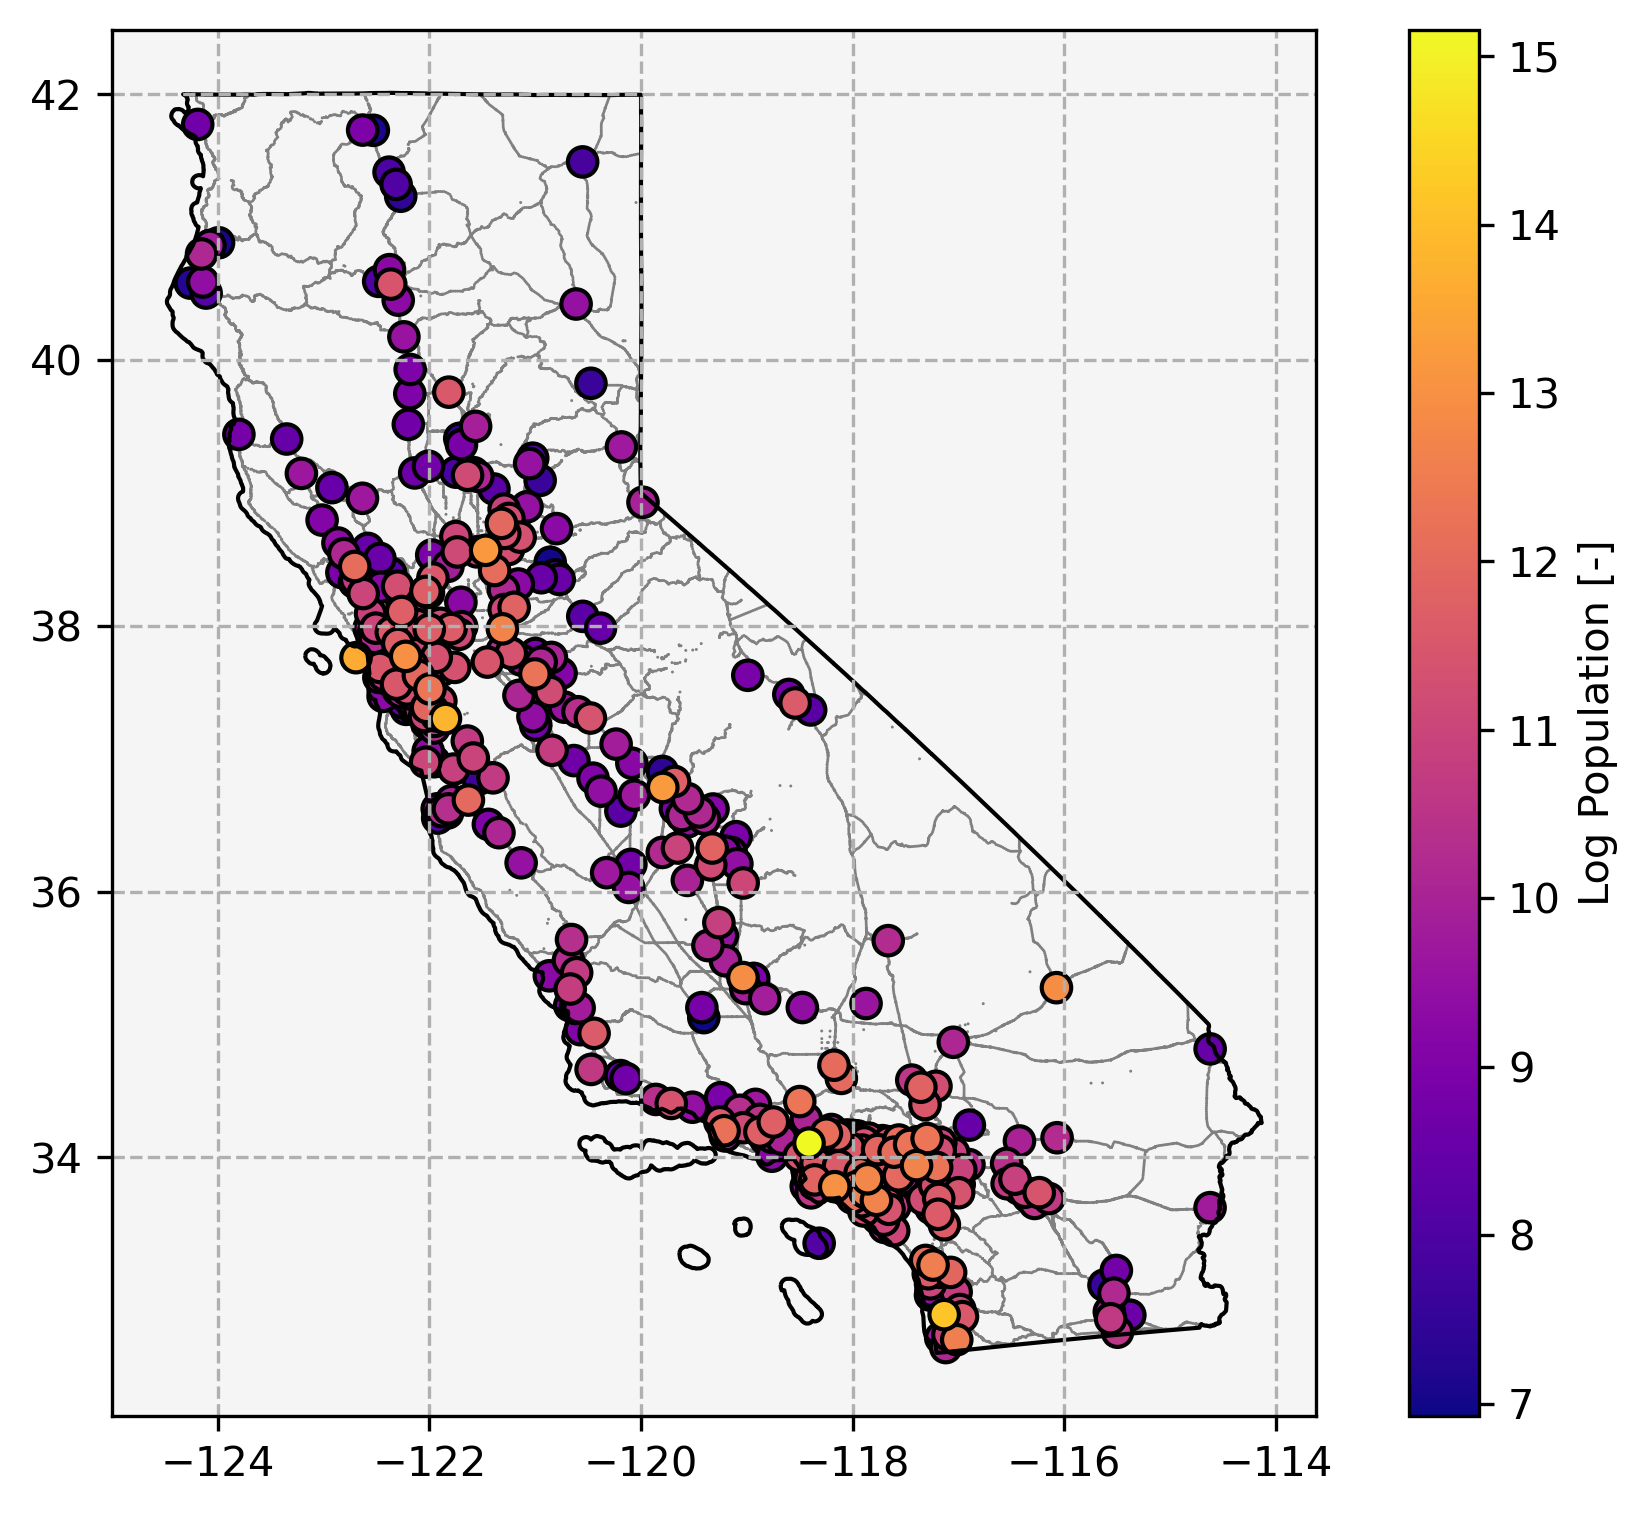
\includegraphics[width = \linewidth]{figs/california_incorporated_places.png}
	\caption{Natural logarithm of population for Incorporated Places in California}
	\label{fig:california_incorporated_places}
\end{figure}

Many of the most heavily populated Places are adjacent with each other or nearly so. The bulk of traffic between these will be local and routine. For the benefit of clarity and brevity these can be merged into super-Places. This is accomplished by the computation of maximally modular communities. First the distances for all pairs are computed. Second an inverse proximity is computed as

\begin{equation}
	\Gamma_{ij} = \exp{\left(\frac{\Phi_d(i,j)}{\epsilon}\right)}
\end{equation}

where $\epsilon$ is a characteristic distance set at 10 km in this case. Solving for maximally modular communities, centroids of the 34 resulting communities are shown in Figure \ref{fig:california_incorporated_communities}.

\begin{figure}[H]
	\centering
	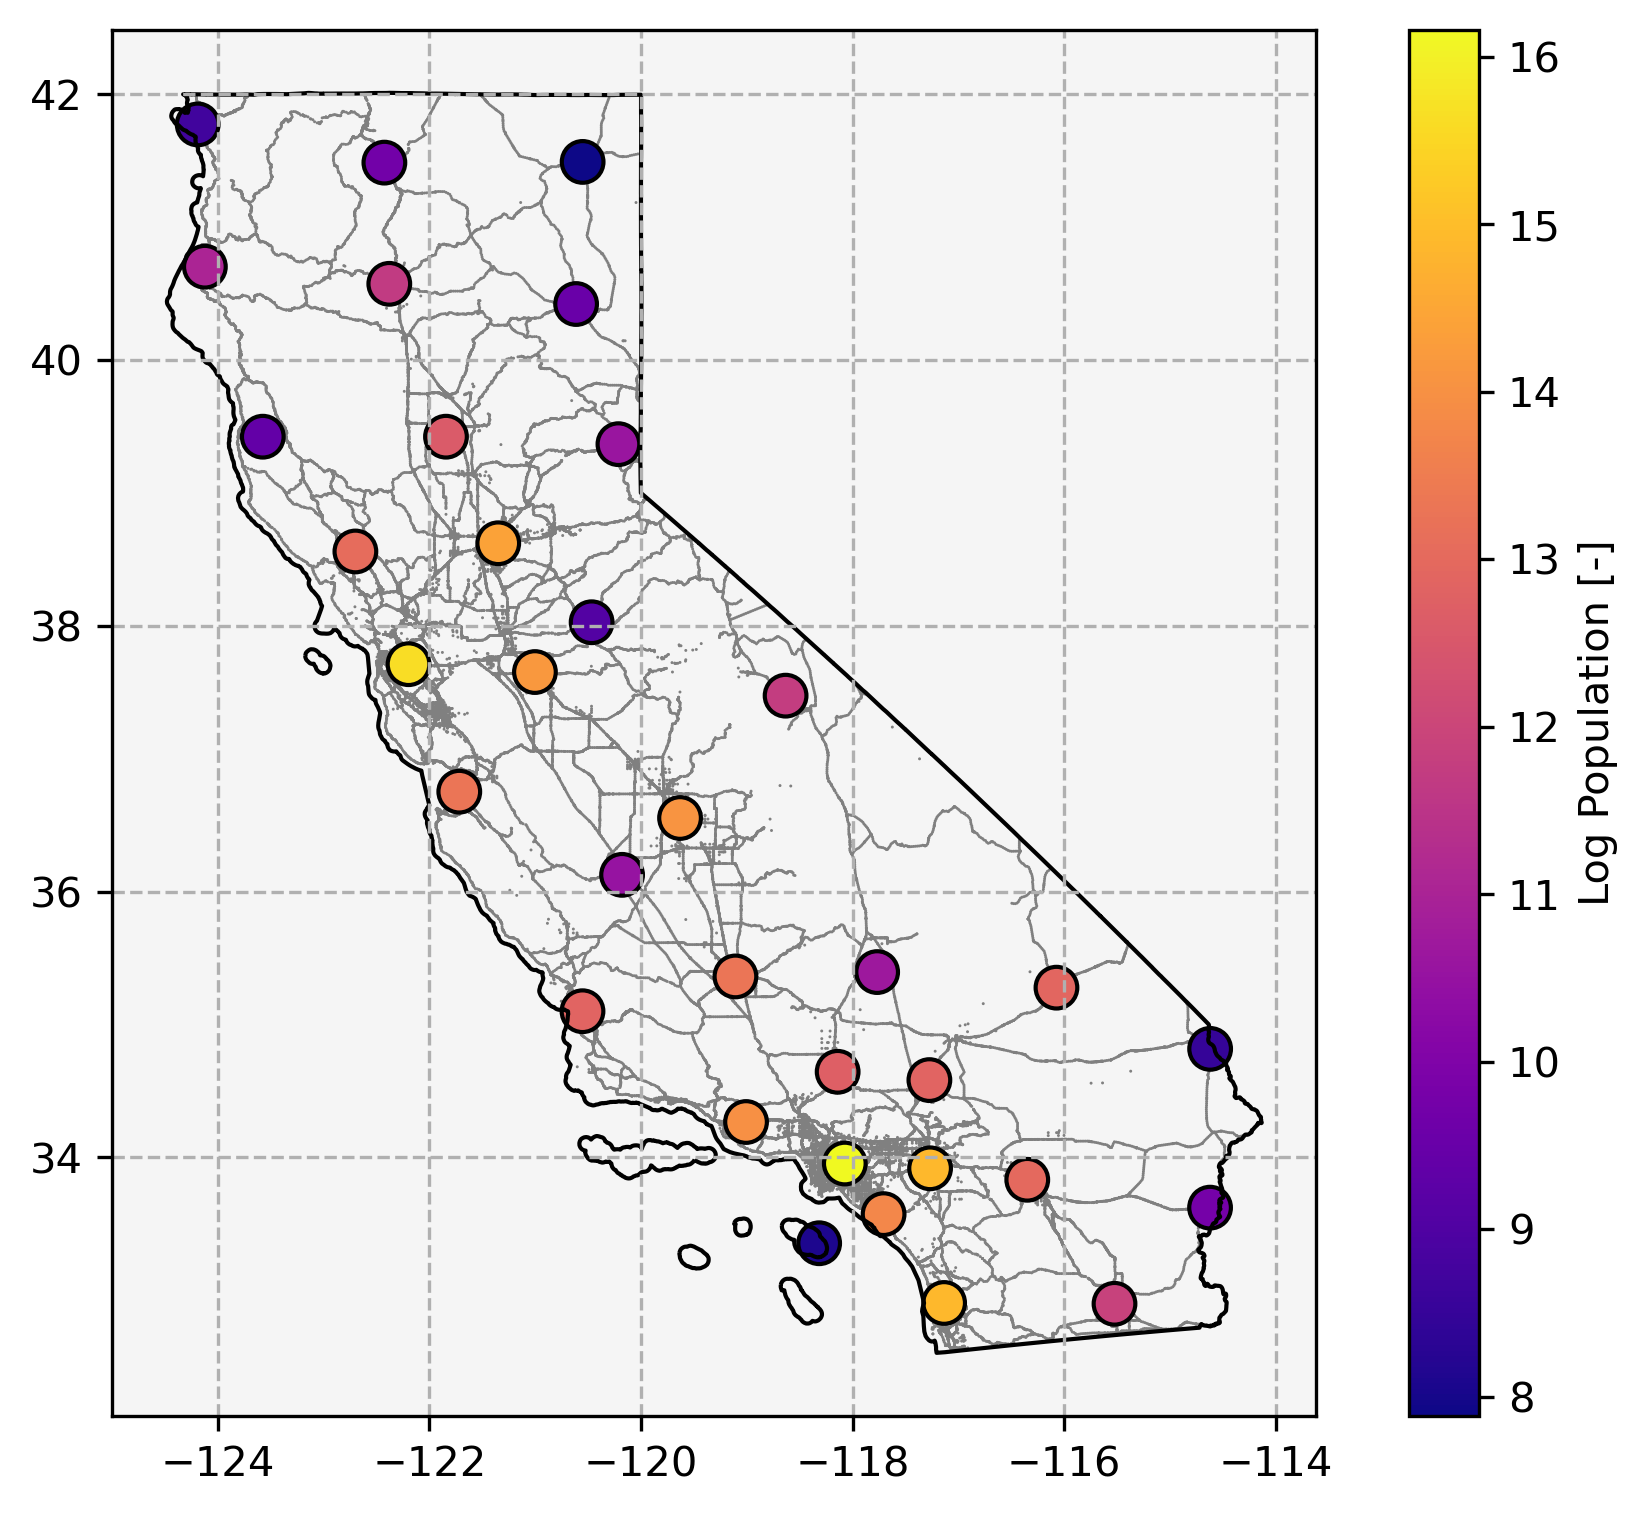
\includegraphics[width = \linewidth]{figs/california_incorporated_communities.png}
	\caption{Natural logarithm  of population for Incorporated Place Communities in California}
	\label{fig:california_incorporated_communities}
\end{figure}

Finally, for the purposes of analysis, points representing departure locations for Phoenix AZ, Las Vegas NV, Reno NV, and Portland/Eugene OR are added to the fringes of the map to represent the associated travel demand.

For long trips, \glspl{bev} will rely on DC charging stations. The locations of all DC charging stations in California are available from AFDC \cite{afdc_2023}. \gls{afdc} is a reasonable but imperfect source for Dc chargers \cite{Xu_2021}. In may 2024 \gls{afdc} listed 2,149 active stations with at least 1 DC charger. This number is somewhat misleading as certain networks report each charger as an individual station even if within line-of-sight of one-another. After merging all stations of the same network which are within 100 meters direct distance of each other the number of stations becomes 1,689. California's DC charging stations include proprietary (vehicle \gls{oem} owned and operated) stations such as Tesla Superchargers and the Rivian Adventure network as well as non-proprietary stations such as those operated by ChargePoint, Electrify America, eVgo, and others. The selected locations and DC charging stations are mapped in Figure \ref{fig:california_stations}.

\end{multicols}

\begin{figure}[H]
\begin{subfigure}{\linewidth/3}
	\centering
	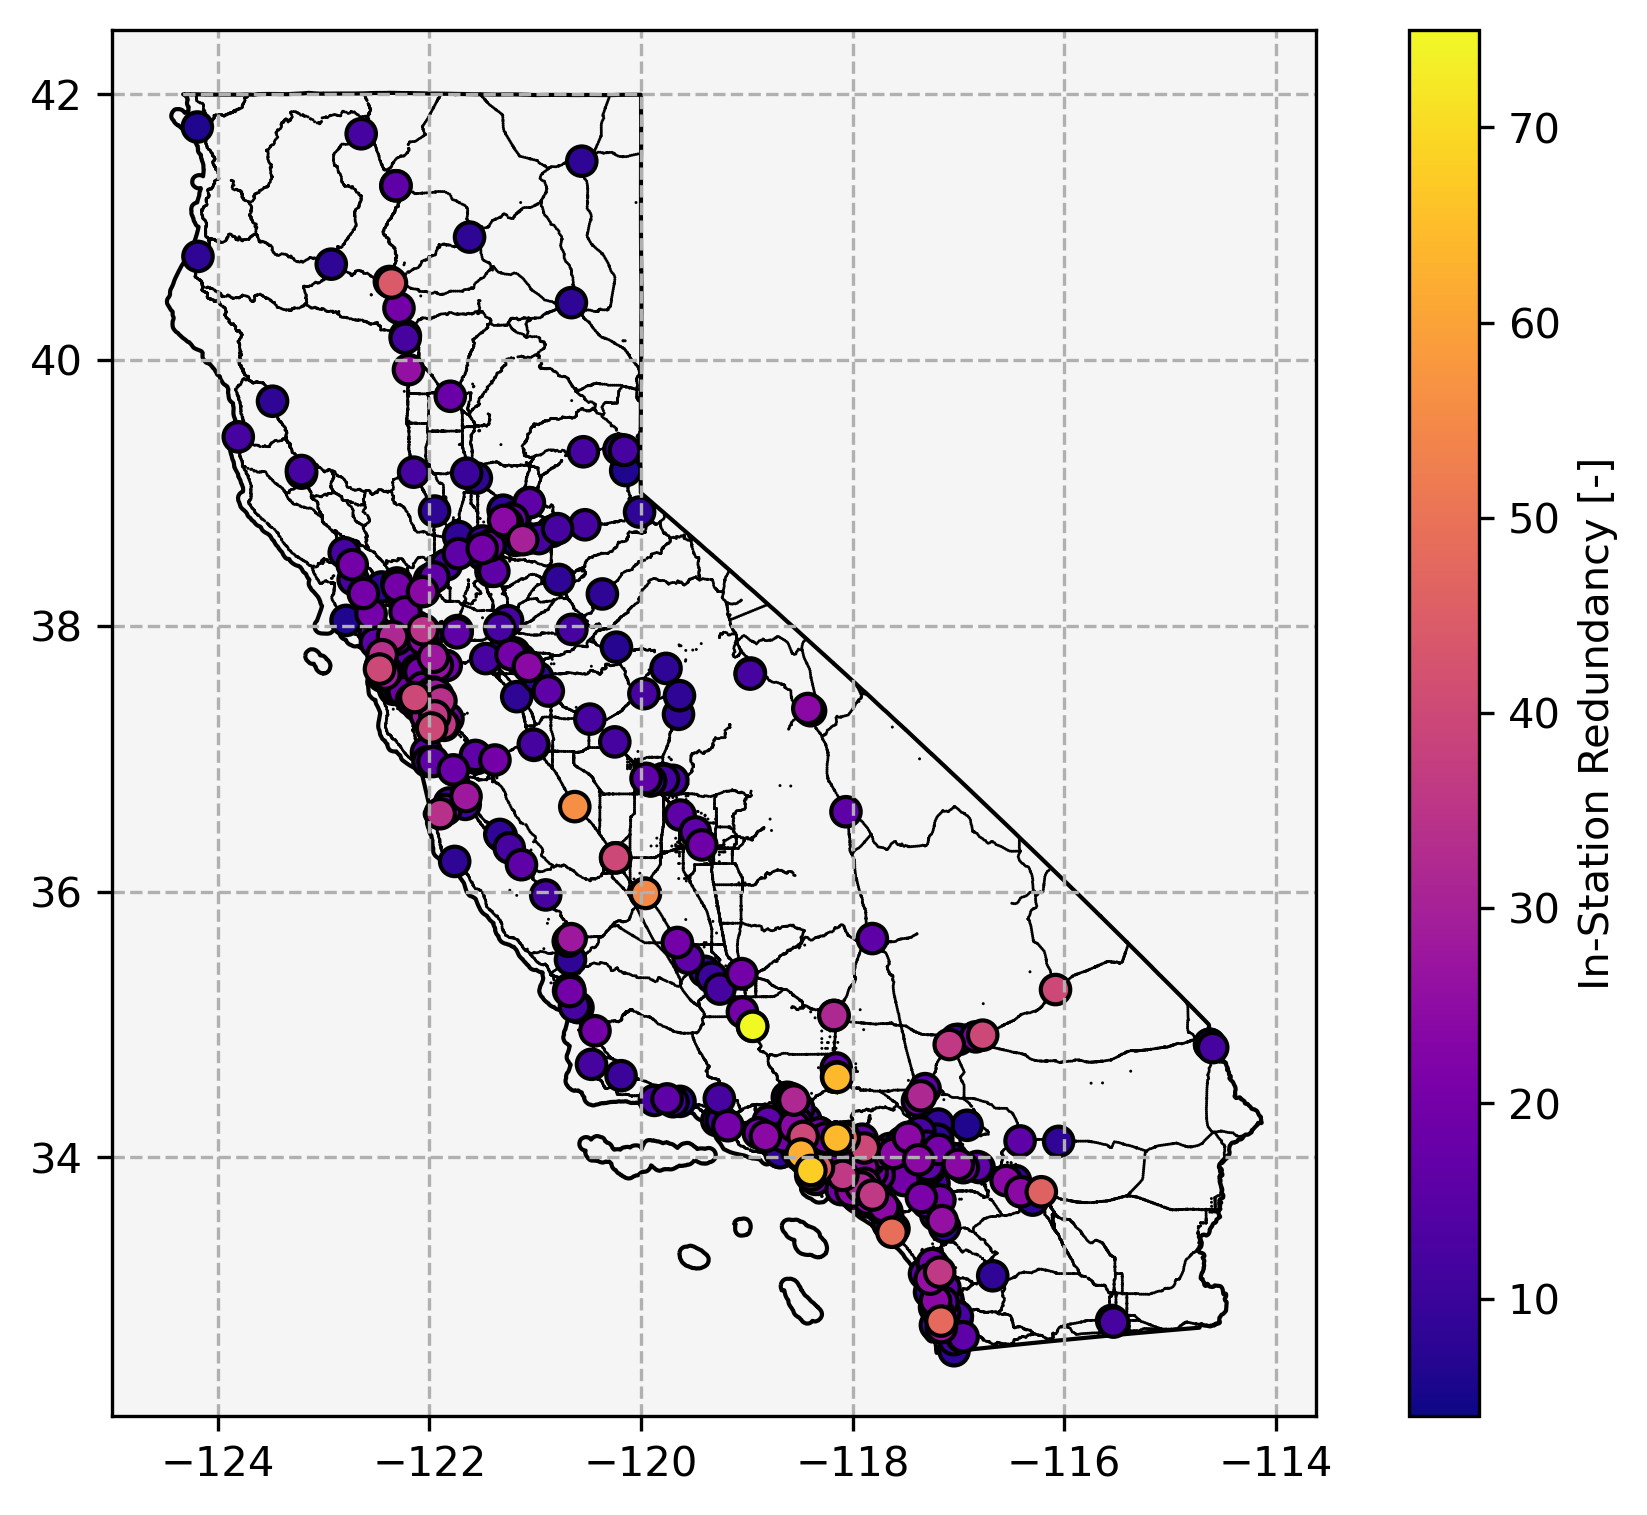
\includegraphics[width = \linewidth]{figs/California_SNG_T.png}
	\caption{Tesla Stations}
\end{subfigure}%
\begin{subfigure}{\linewidth/3}
	\centering
	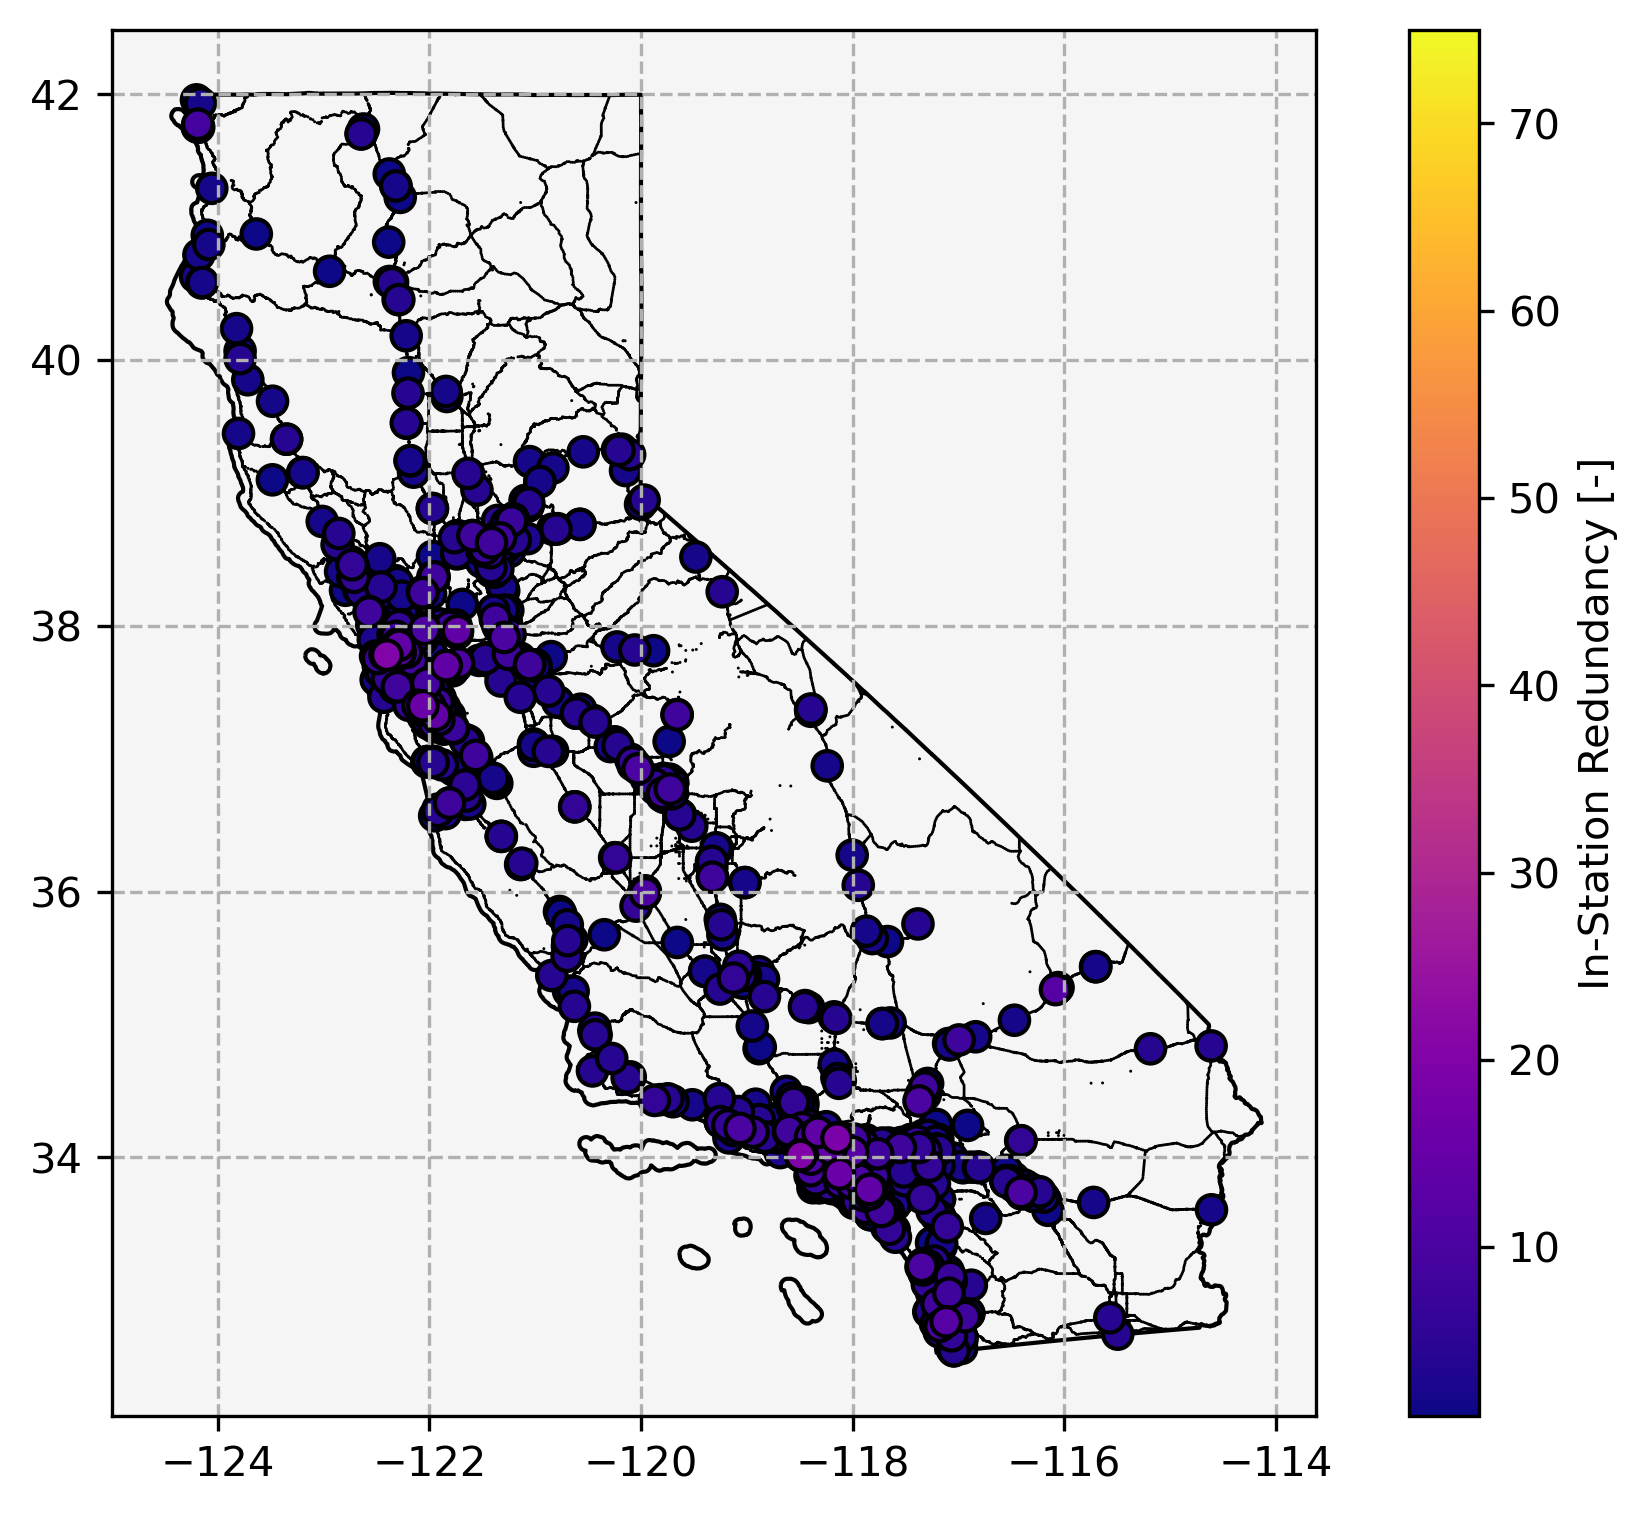
\includegraphics[width = \linewidth]{figs/California_SNG_NT.png}
	\caption{Non-Tesla Stations}
\end{subfigure}
\begin{subfigure}{\linewidth/3}
	\centering
	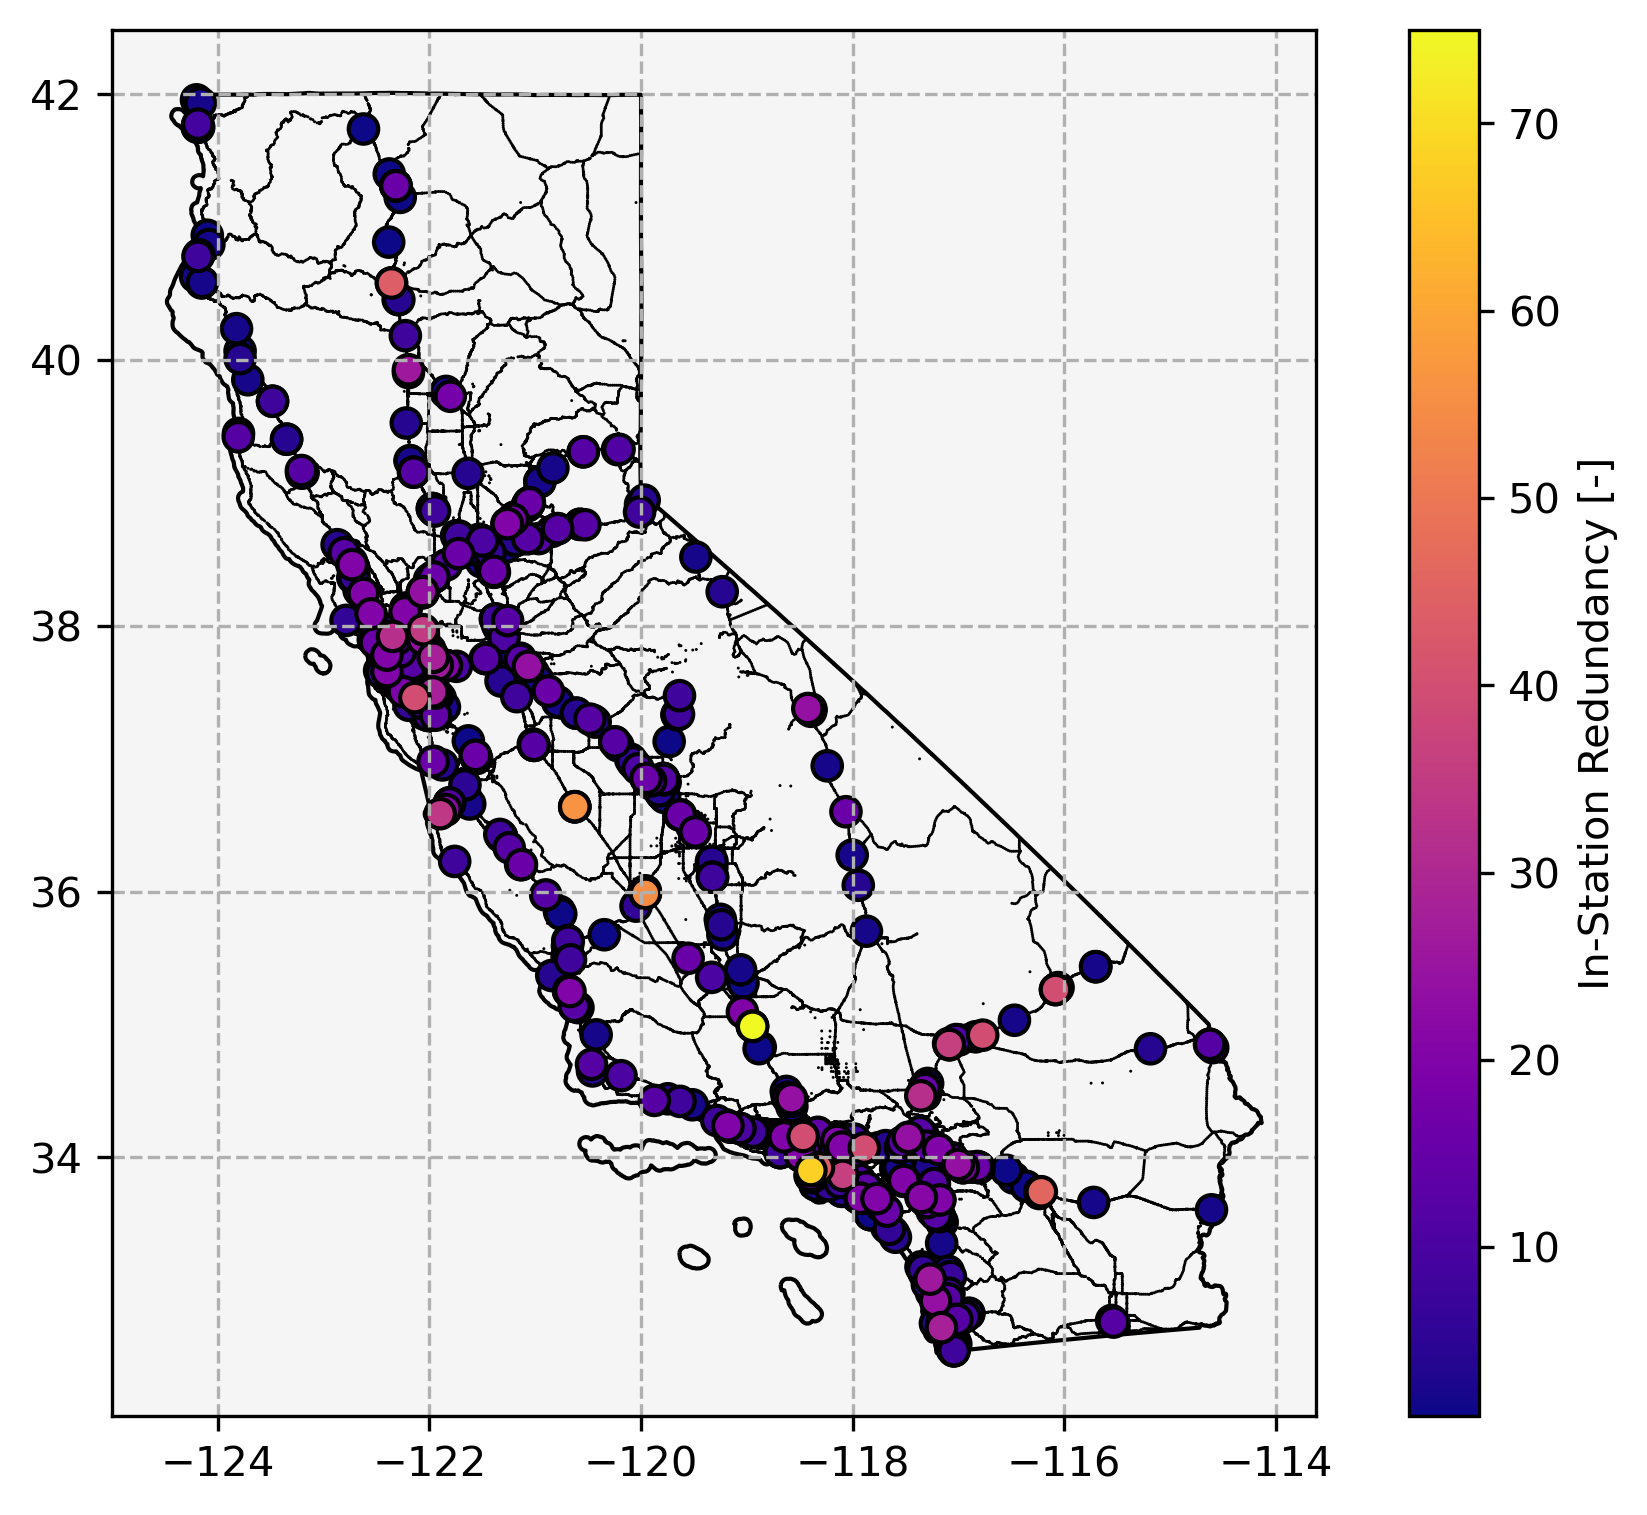
\includegraphics[width = \linewidth]{figs/California_SNG_C.png}
	\caption{Corridor Stations}
\end{subfigure}
\caption{California DC charging stations from \gls{afdc} (May 2024)}
\label{fig:california_stations}
\end{figure}

\begin{multicols}{2}

There are 419 Tesla and 16 Rivian DC charging stations in the state as compared to 1,254 non-proprietary DC charging stations. In practice, many of these stations will be of little use for long distance travel being located far away from primary and secondary roads. Considering only those stations within 1 km of a highway as "corridor" chargers, there are a total of 500 corridor DC charging stations. Of the corridor stations, 156 are Tesla stations, 7 are Rivian stations, and 344 are non-Proprietary stations.

The non-Tesla networks overwhelmingly use CCS or combination CCS/ChaDeMo chargers which reflect the ports on the overwhelming number of non-Tesla \glspl{bev}. By contrast, Tesla chargers and vehicles use the NACS standard. The Tesla and non-Tesla systems are historically separate but increasingly interoperable with the aid of adapters. Tesla drivers use Tesla DC chargers almost exclusively \cite{Visaria_2022}. The Rivian Adventure network is technically interoperable with other J1772 vehicles but is set aside for the exclusive use of Rivian vehicles. The purpose of the Rivian Adventure network serves to allow for Rivian vehicles to charge in remote locations and is not intended to be relied upon exclusively.

The difference between the Tesla DC charging network and the non-Tesla networks extends from function to form. Built out as an investment to entice sales of Tesla vehicles and, until recently, exclusive to them, the Tesla network is technically superior with high maximum charging rates and more greater port usability rates \cite{Rempel_2023, Kozumplik_2022}. The Tesla network is mainly composed of high redundancy stations. Non-proprietary networks have, so far, been utilization and subsidy driven \cite{Gamage_2023} and are widely distributed with low redundancy stations. A stark contrast is seen when examining the ratios of chargers to stations. In California there are 403 Tesla DC charging stations with a total of 7,101 DC chargers for an average of 16.9 chargers per station. Among non-proprietary networks there are a total of 1,254 stations with 4,129 chargers for an average of 3.3 per station. Redundancies for Tesla and non-proprietary networks are shown in Figure \ref{fig:network_histograms}. 


\begin{figure}[H]
	\centering
	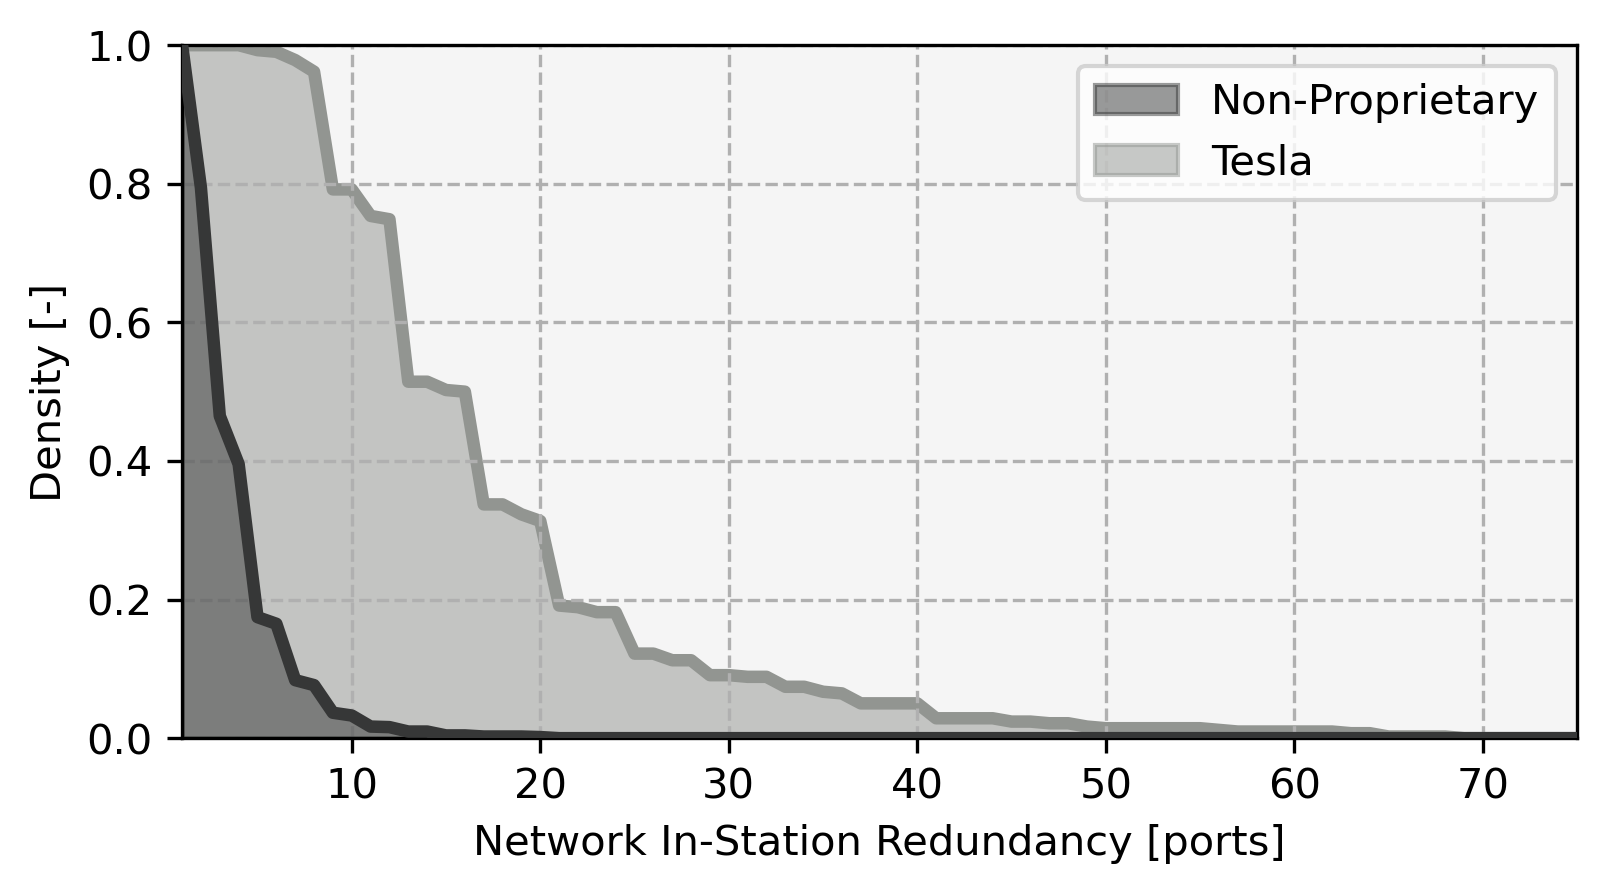
\includegraphics[width = \linewidth]{figs/California_RIS_Hist.png}
	\caption{Survival functions for in-station redundancy for Tesla and other DC charger networks in California}
	\label{fig:network_histograms}
\end{figure}

The Tesla DC charging network develops redundancy primarily in-station where the non-proprietary networks develop redundancy primarily between stations. Non-Tesla chargers are also more likely to be sighted in urban areas suggesting a desire to capture local as well as corridor travel demand. Tesla stations are more often sighted along travel corridors suggesting a focus on enabling long distance travel. In more remote parts of California the proprietary networks nearly match the non-proprietary networks in station numbers. In-station redundancies for DC charging networks in California can be found in Figures in the DC Charger Network Details section of the Appendix. Summary statistics for DC charging networks in California can be found in the DC Charger Network Details section of the appendix.

California \glspl{icev} utilize a third and completely separate network of supply stations. There are estimated to be over 8,000 gasoline stations in California \cite{CEC_2022} and these are widely and proportionally distributed. Because no public database for the locations of gasoline stations in the state exists, and due to their ubiquity it is assumed in this study that \gls{icev} driver optimal paths will not be effected by fueling station availability. For this reason, \glspl{icev} are, herein, assumed to take the "direct" path between cities where \glspl{bev} need to find optimal paths on their \glspl{sng}.

\subsection*{Experiment}

In order to understand the effects of vehicular, infrastructural, and behavioral parameters on road-trip accessibility an experiment was carried out on randomly generated combinations. As a baseline, three \glspl{icev} were also modeled. These \glspl{icev} represent different levels of efficiency present in the \gls{icev} fleet. The \gls{icev} models use \gls{ess} capacity numbers are pulled from manufacturer websites and energy consumption rates from \cite{DOE_EPA_2024}. Although substantially less efficient than equivalent \glspl{bev} the comparatively high specific energy of liquid petroleum allows for \glspl{icev} to have high full-tank ranges. \gls{icev} supply infrastructure is modeled to dispense fuel at the normal US rate of 7 gallons per minute which is an equivalent energy supply rate of 14.15 MW. When refueling, the Prius. Golf, and Pacifica, add highway range at rates of 631, 462, and 282 km per minute respectively. The \gls{icev} models are shown in Table \ref{tab:icev_models}.
	
\begin{table}[H]
	\centering
	\caption{\gls{icev} models}
	\label{tab:icev_models}
	\begin{tabular}{|C{.4\linewidth}|C{.35\linewidth}|C{.25\linewidth}|}
		\hline \rowcolor{lightgray} Vehicle Model & Parameter & Value \\
		\hline & \gls{ess} Capacity & 381 [kWh] \\
		\cline{2-3} 2024 Toyota Prius & Energy Consumption & 1,346 [kJ/km] \\
		\cline{2-3} & Full-Tank Range & 1,018 [km] \\
		\cline{1-3} & \gls{ess} Capacity & 445 [kWh] \\
		\cline{2-3} 2024 Volkswagen Golf & Energy Consumption & 1,839 [kJ/km] \\
		\cline{2-3} & Full-Tank Range & 871 [km] \\
		\cline{1-3} & \gls{ess} Capacity & 640 [kWh] \\
		\cline{2-3} 2024 Chrysler Pacifica & Energy Consumption & 3,015 [kJ/kM] \\
		\cline{2-3} & Full-Tank Range & 764 [km] \\
		\hline
	\end{tabular}
\end{table}

Regional Impedance for \glspl{icev} was computed under the assumption of petroleum supply infrastructure ubiquity. As such, \glspl{icev} were given the "direct" path between locations with stop times added where additional range was needed. For each necessary stop, time was added for refueling to full as well as 10 minutes to divert from the road and handle the transaction prior to refueling. Additionally, drivers of the \glspl{icev} were assumed to keep a 10\% buffer of remaining range. The \glspl{icev} each had similar road-trip accessibility scores of roughly 5.5 hours. The longest arc considered in Crescent City (Location 0) to Phoenix - State Line (Location 13) which is roughly 1,530 km just exceeding double the usable range of the Pacifica.

500 random scenarios were generated by uniform random sampling of the parameters listed in Table \ref{tab:experimental_parameters} and run on three \glspl{sng} as described in \ref{tab:experimental_sngs}. All randomly sampled \glspl{bev} in this study are assumed to have an energy consumption rate of 608 kJ/km this being the EPA energy consumption rate of a Tesla Model 3 in highway operation \cite{DOE_EPA_2024}. Highway operation is assumed herein due to the focus on long trips. Thus \gls{bev} full-charge ranges will be between 237 and 711 km. When charging, sampled \glspl{bev} add highway range at a rate between 4.9 and 19.7 km per minute. Risk attitude is modeled as in \eqref{eq:superquantile} with the range centered around the mean parameter $\overline{p}$ where $p_0 = \overline{p} - .1$ and $p_1 = \overline{p} + .1$. 

\begin{table}[H]
	\centering
	\caption{Parameters and ranges for experiment.}
	\label{tab:experimental_parameters}
	\begin{tabular}{|C{\linewidth/2}|C{\linewidth/2}|}
		\hline \rowcolor{lightgray} Parameter & Range \\
		\hline \gls{ess} Capacity & [40 kWh, 120 kWh] \\
		\hline \gls{ess} Max Charge Rate & [50 kW, 200 kW] \\
		\hline Driver Risk-Attitude Mean & [.1, .9] \\
		\hline \gls{evse} Reliability & [.5, 1] \\
		\hline
	\end{tabular}
\end{table}

\begin{table}[H]
	\centering
	\caption{\glspl{sng} used in experiment.}
	\label{tab:experimental_sngs}
	\begin{tabular}{|C{\linewidth/3}|C{\linewidth*2/3}|}
		\hline \rowcolor{lightgray} Label & Networks Included \\
		\hline Combined & All stations \\
		\hline Tesla & Only Tesla stations \\
		\hline Non-Tesla & All non-Tesla stations \\
		\hline
	\end{tabular}
\end{table}

Outputs were processed to compute neutral expectations of Regional Gravity and Regional Impedance as in \eqref{eq:regional_gravity} and \eqref{eq:regional_impedance} respectively. Boxplots of Regional Gravity and Regional Impedance by \gls{sng} are presented in Figures \ref{fig:networks_boxplots_gravity} and \ref{fig:networks_boxplots_impedance}.

\begin{figure}[H]
	\centering
	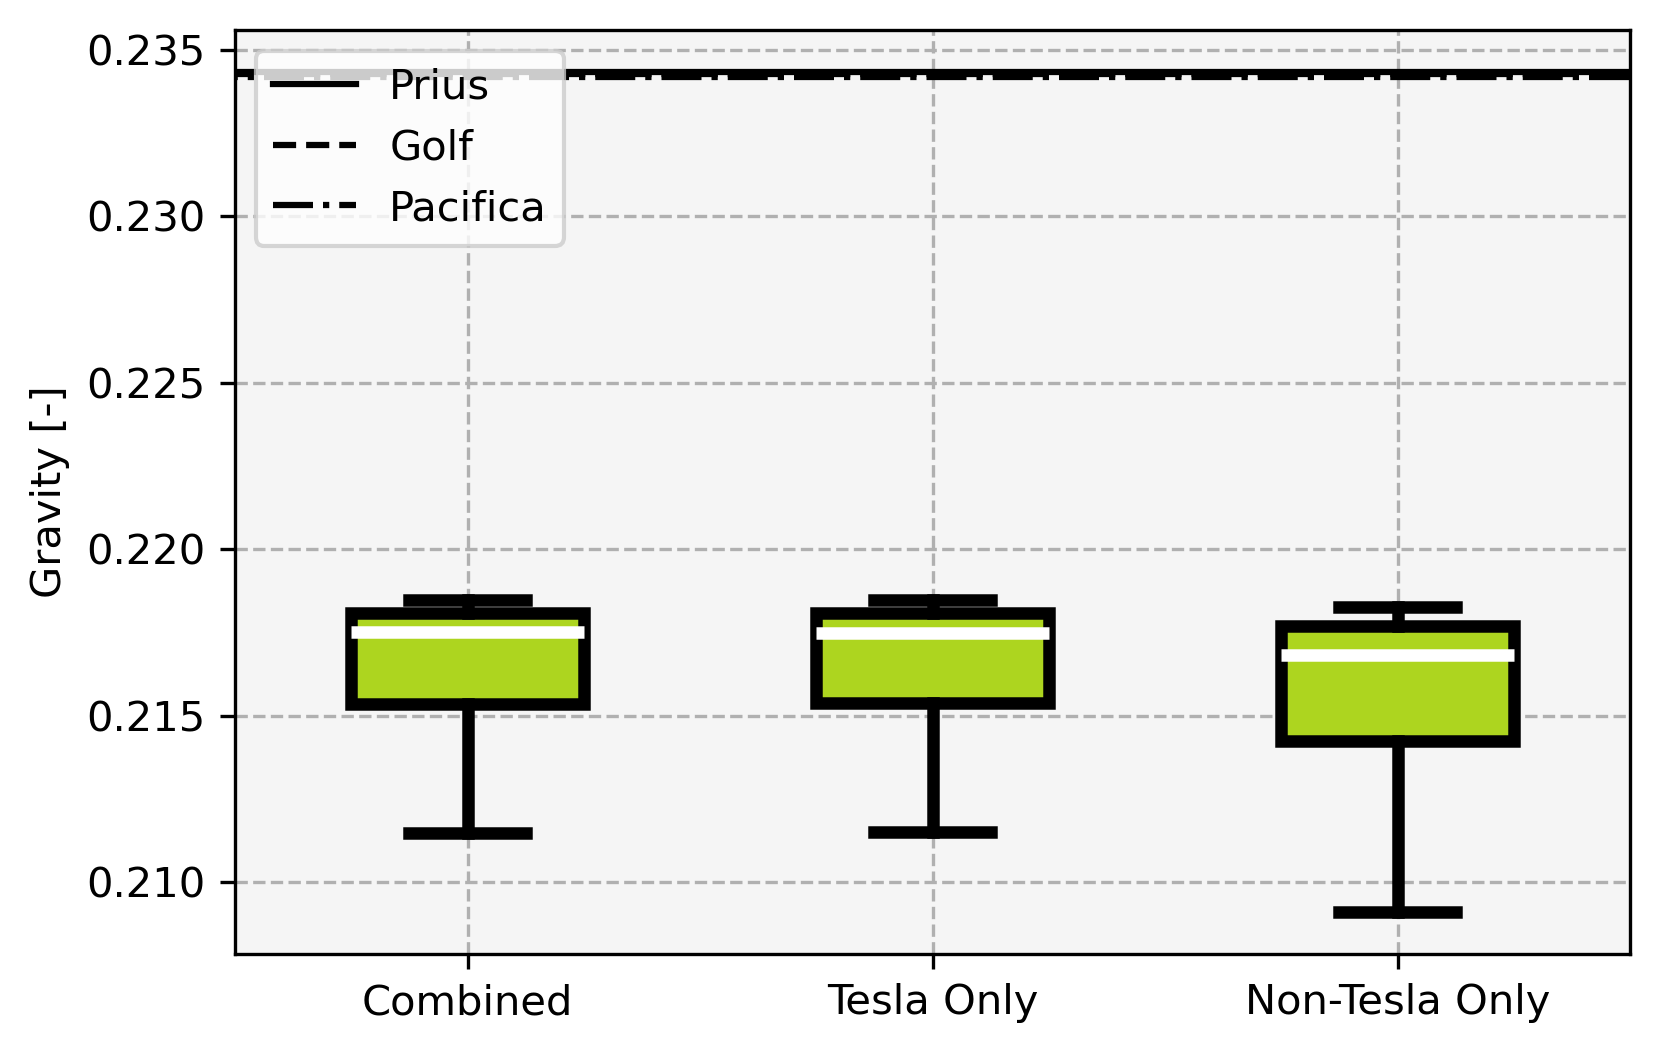
\includegraphics[width = \linewidth]{figs/Networks_Boxplots_Gravity.png}
	\caption{Boxplots of $G_R$ outputs by \gls{sng}}
	\label{fig:networks_boxplots_gravity}
\end{figure}

\begin{figure}[H]
	\centering
	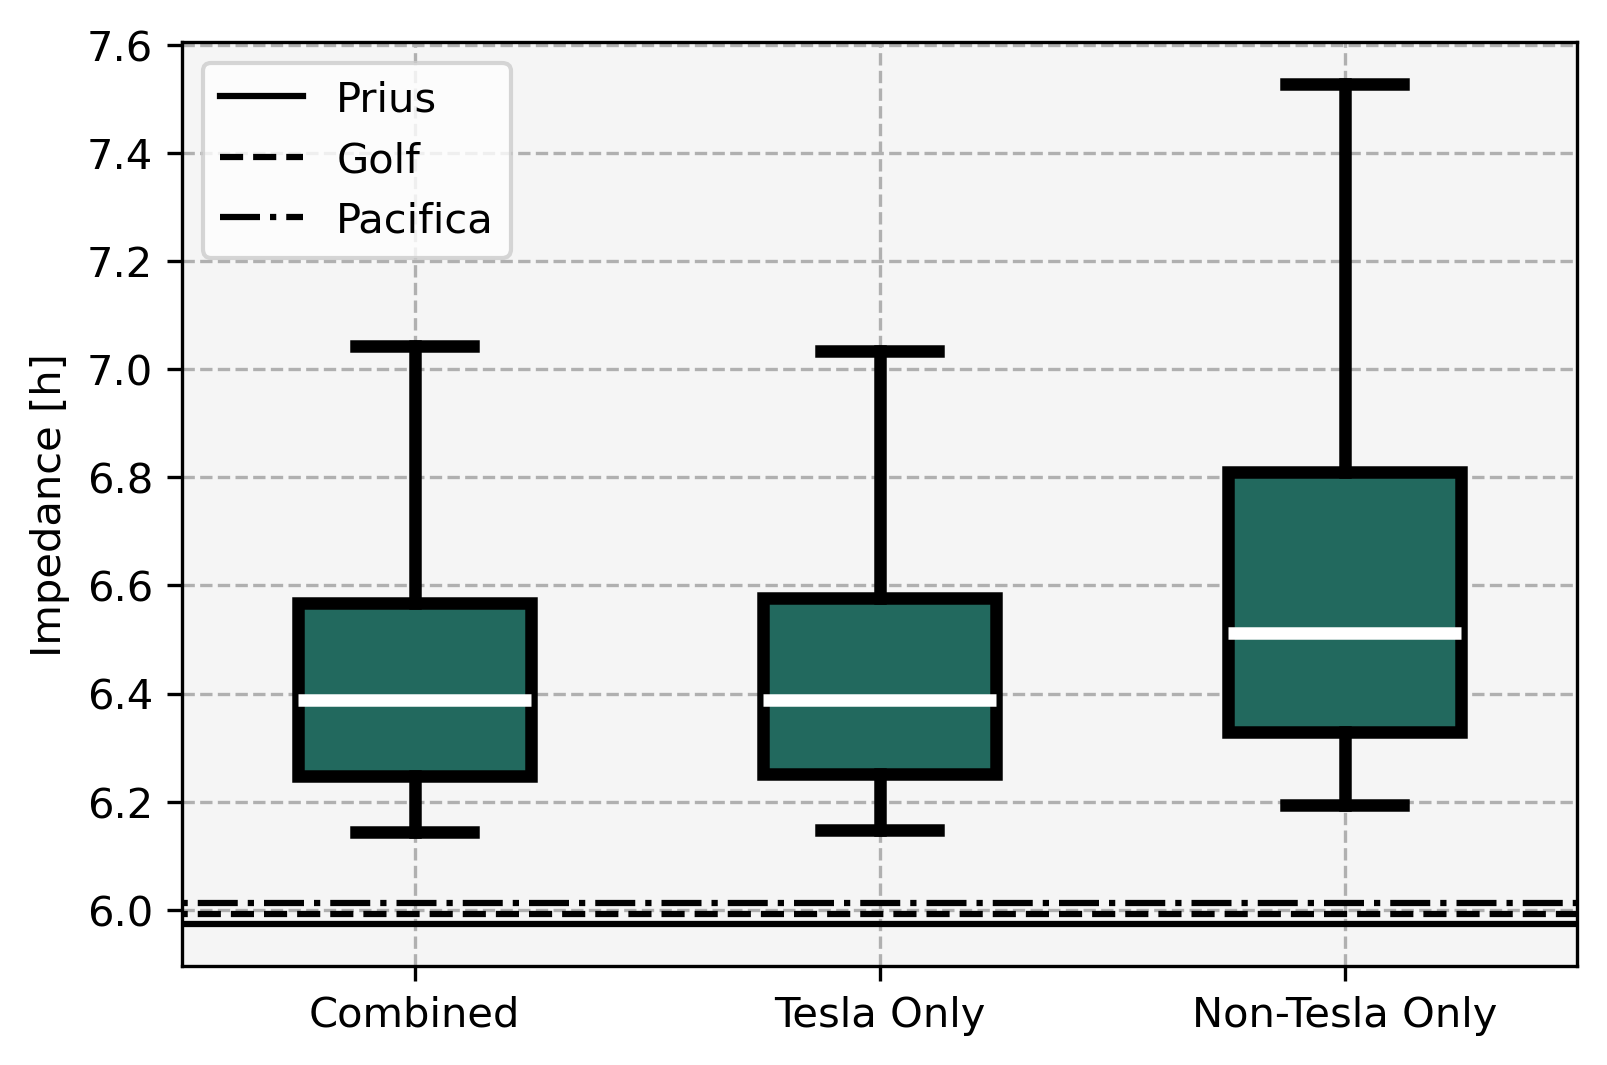
\includegraphics[width = \linewidth]{figs/Networks_Boxplots_Impedance.png}
	\caption{Boxplots of $Z_R$ outputs by \gls{sng}}
	\label{fig:networks_boxplots_impedance}
\end{figure}

An immediate takeaway is the value of access to Tesla stations. The median performance of the Tesla \gls{sng} is only very slightly worse than that of the complete \gls{sng} while the performance of the non-Tesla \gls{sng} is notably worse than either. The outcome spread among the sampled cases is substantial ranging from marginally worse than the \glspl{icev} to markedly worse. As gravity scales with the inverse of the square of impedance it follows that, purely from a road transportation perspective, the current \gls{bev} infrastructure would result in a noticeably less connected region. The bulk of the increase in impedance occurs at-station whether due to queuing or charging times. Although statistically significant, the time lost due to path deviations is minimal as seen in Figure \ref{fig:networks_boxplots_driving}.

\begin{figure}[H]
	\centering
	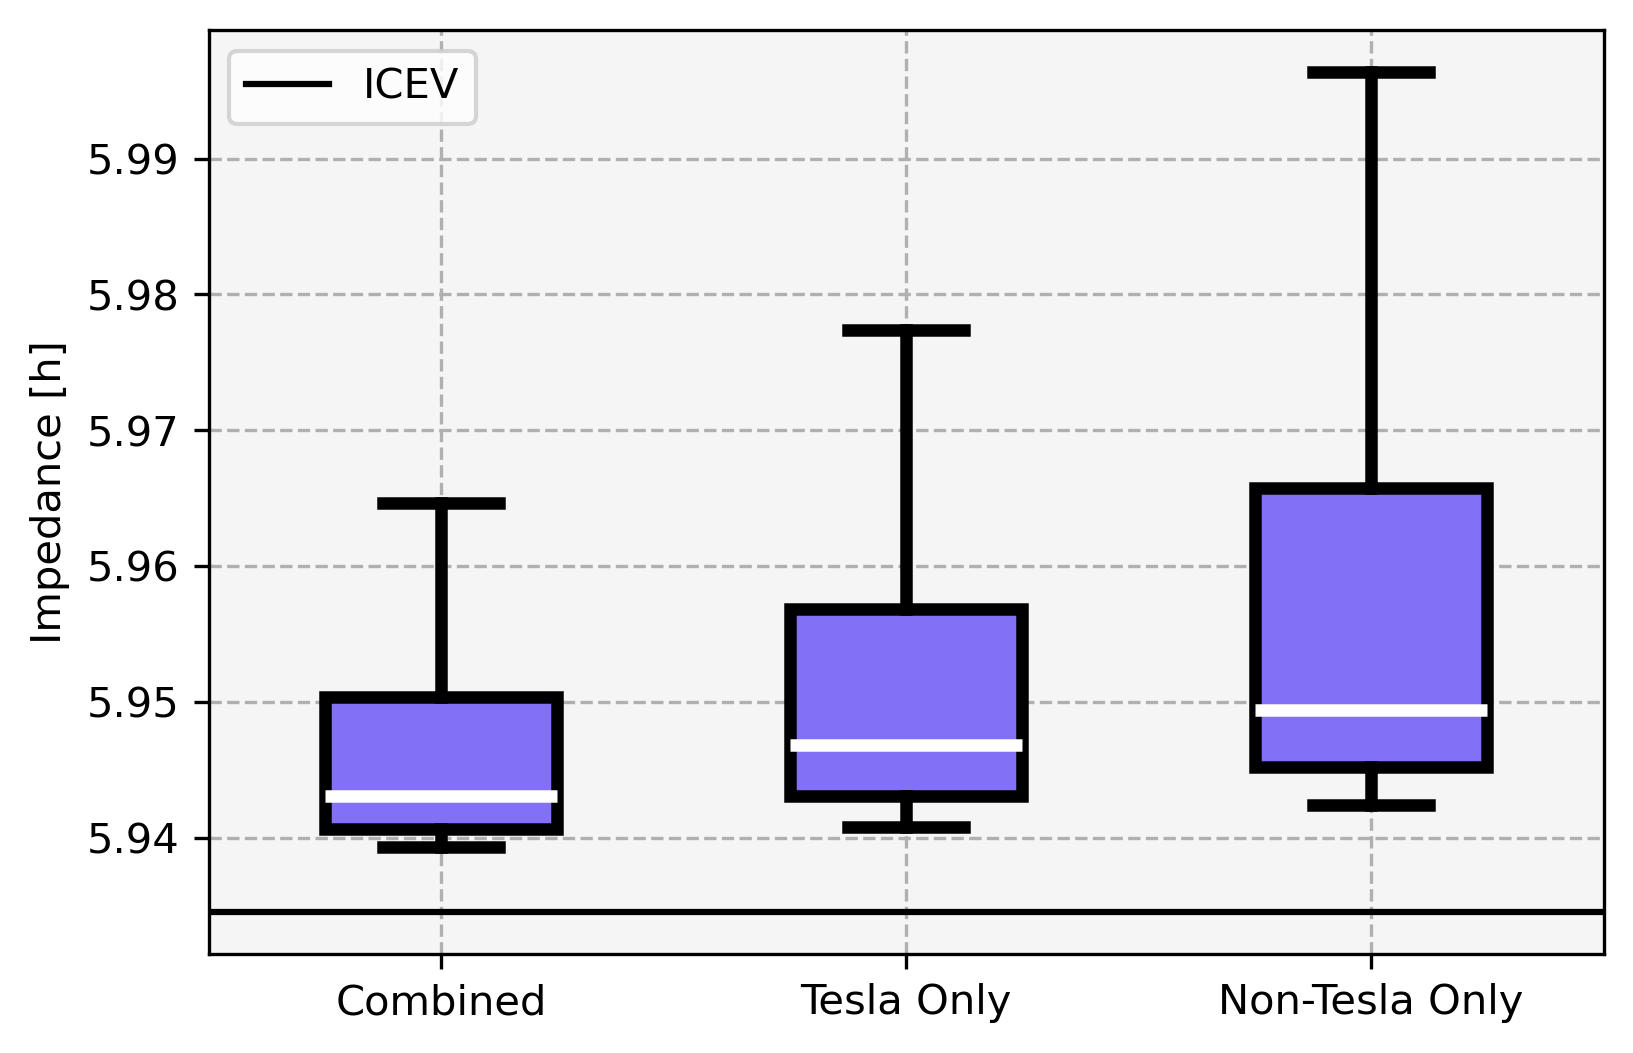
\includegraphics[width = \linewidth]{figs/Networks_Boxplots_Impedance_Driving.png}
	\caption{Boxplots of $Z_R$ outputs by \gls{sng} neglecting supply time}
	\label{fig:networks_boxplots_driving}
\end{figure}

Having identified the effects of \gls{sng}, the effects of vehicular and behavioral parameters on experience for the given \glspl{sng} can be identified. Linear regression was performed on the Regional Impedance results of the random experiment and the experimental parameters for each \gls{sng}. Significant parameters from the regression are shown in Figure \ref{fig:significant_parameters_0}. Regression details are tabulated in the Regression Details section of the Appendix. 

\end{multicols}

\begin{figure}[H]
	\centering

\begin{subfigure}[t]{.33\linewidth}
	\centering\captionsetup{width = .8\linewidth}
	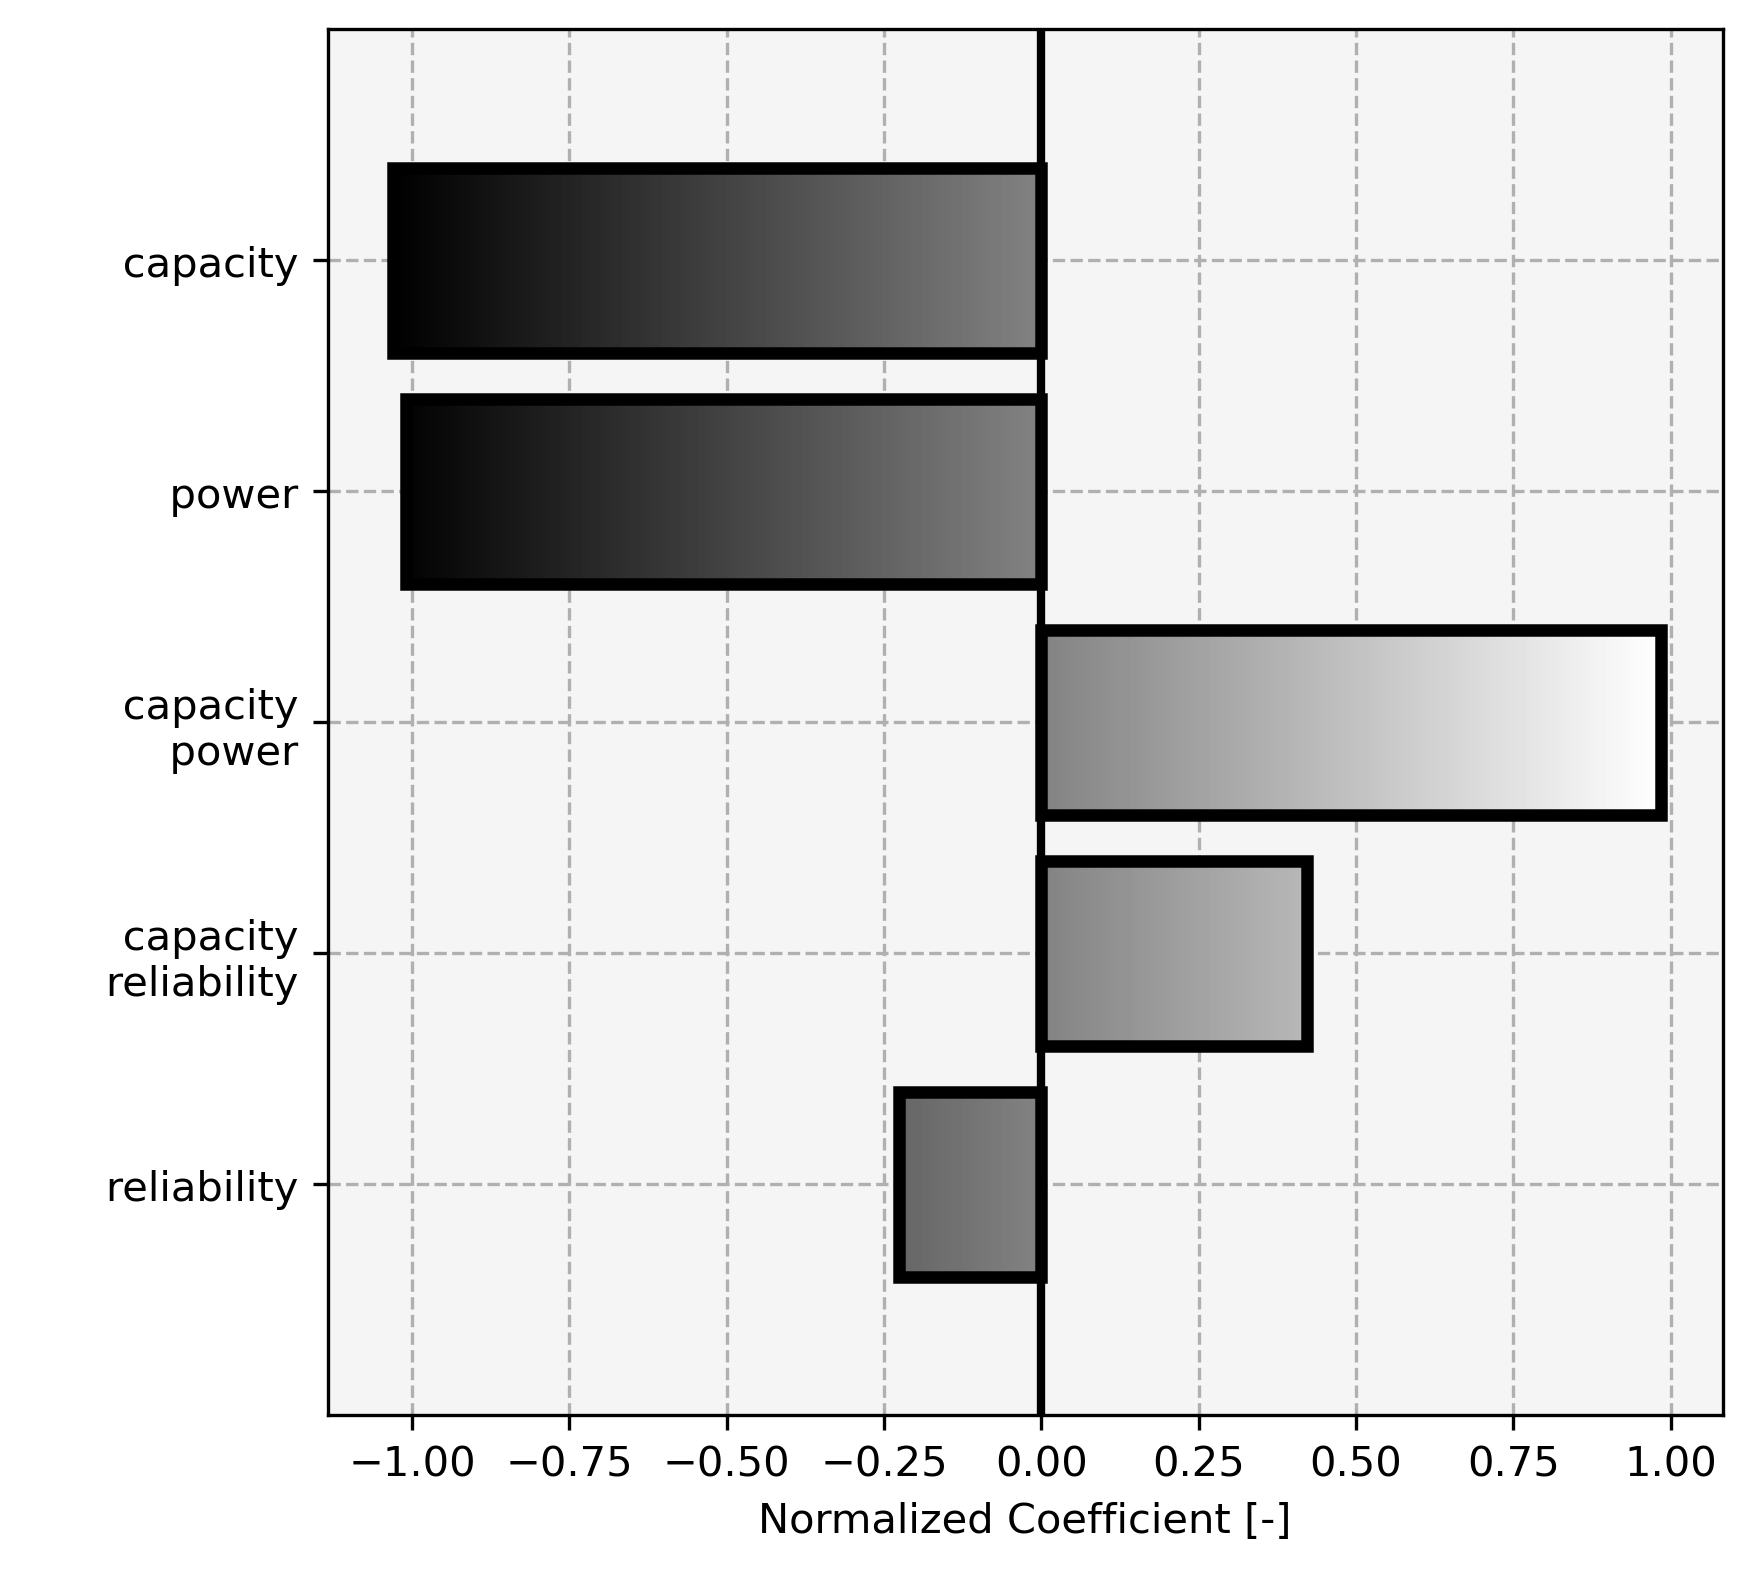
\includegraphics[width = \linewidth]{figs/significant_parameters_0.png}
	\caption{Complete network}
\end{subfigure}%
\begin{subfigure}[t]{.33\linewidth}
	\centering\captionsetup{width = .8\linewidth}
	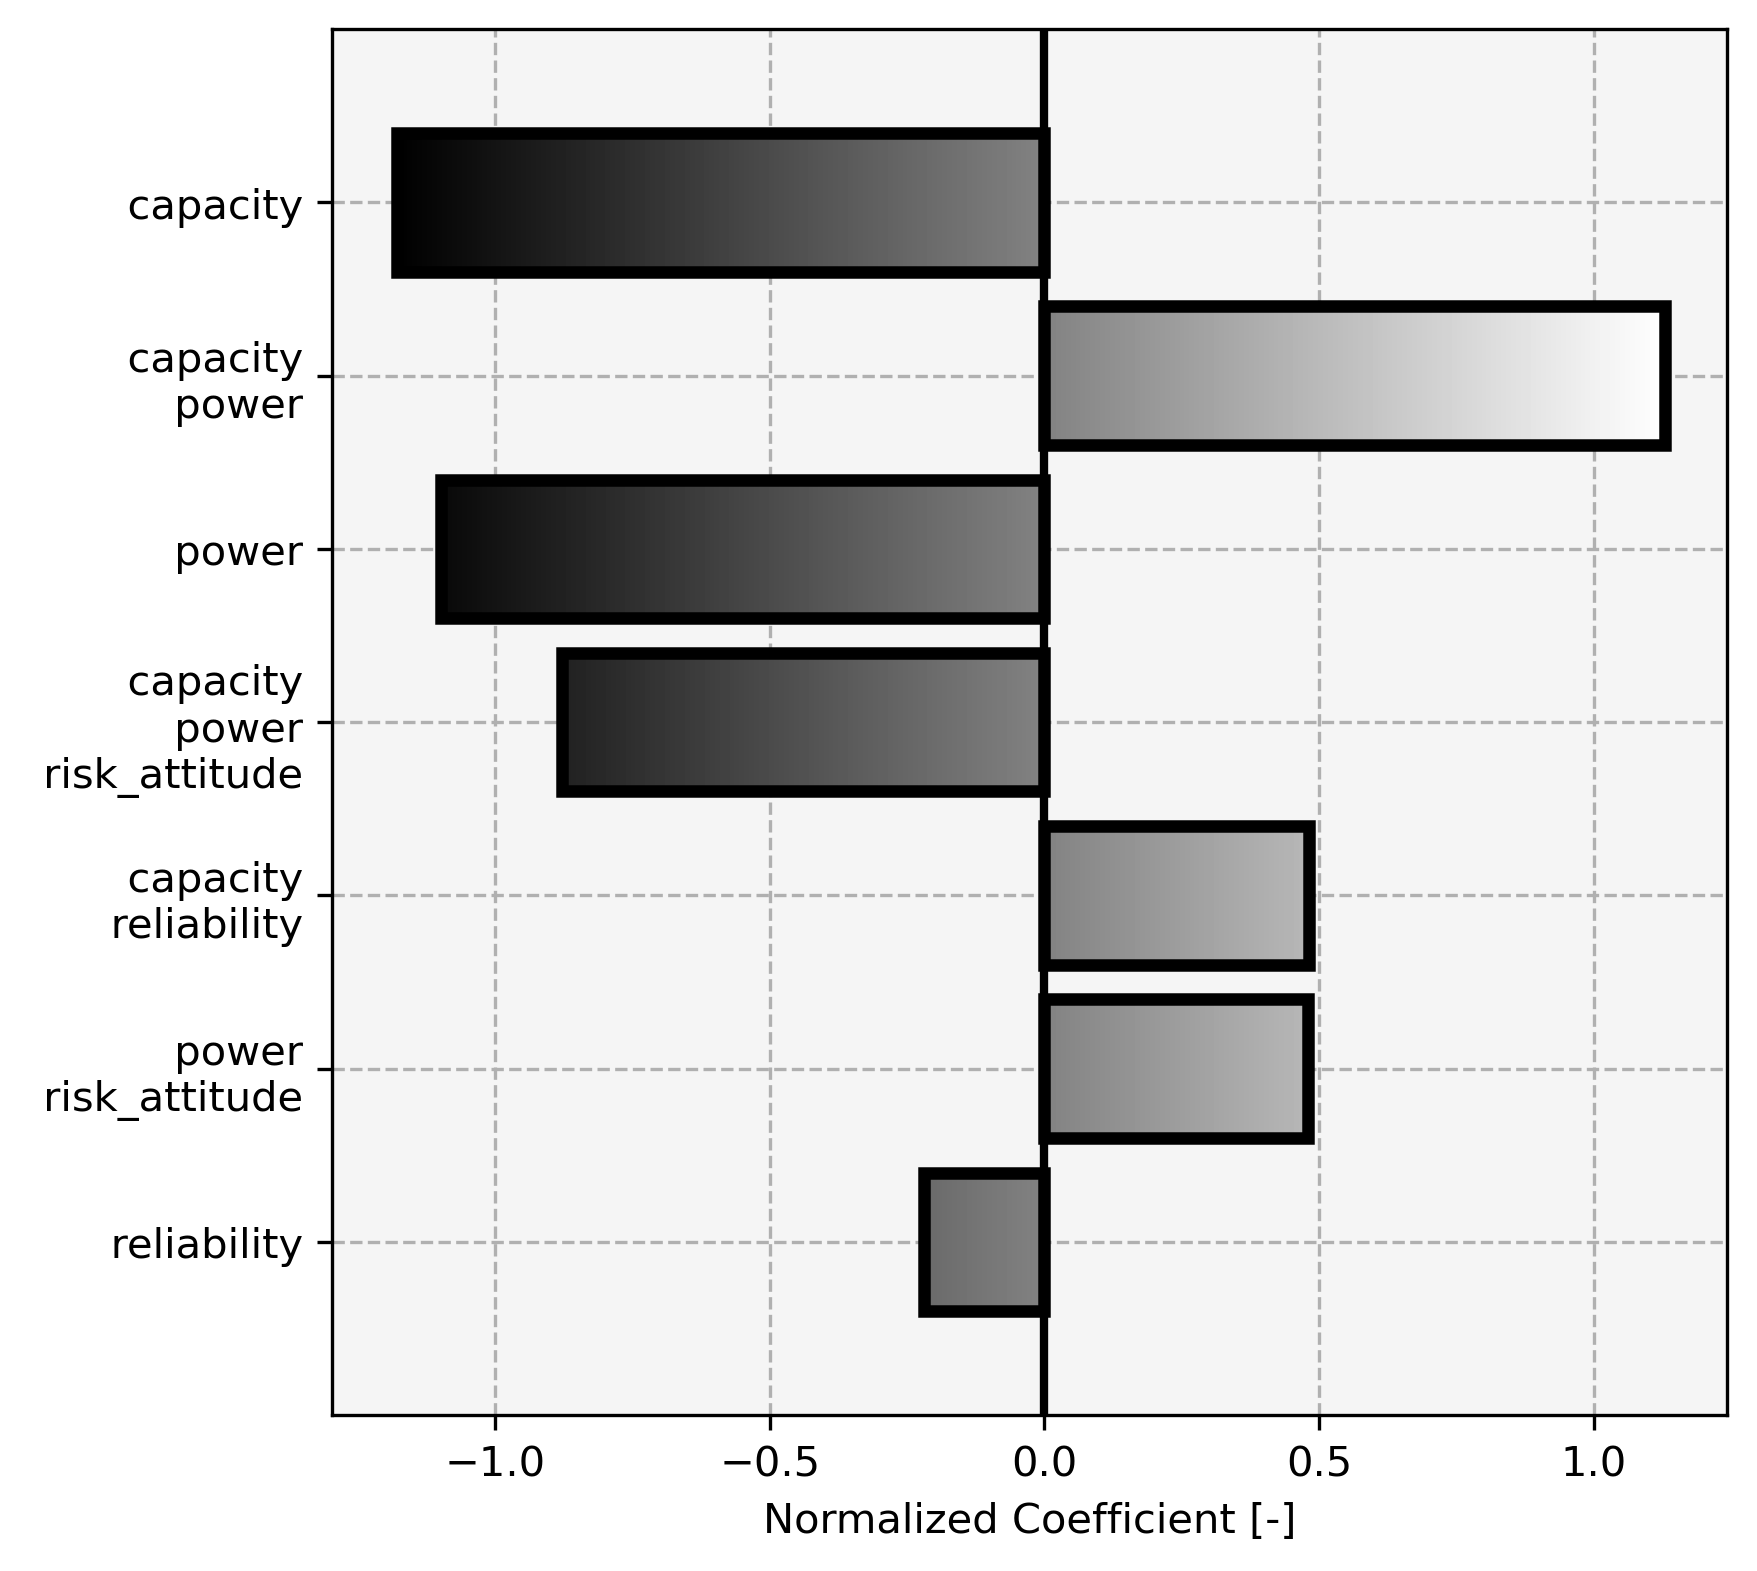
\includegraphics[width = \linewidth]{figs/significant_parameters_1.png}
	\caption{Tesla stations only}
\end{subfigure}%
\begin{subfigure}[t]{.33\linewidth}
	\centering\captionsetup{width = .8\linewidth}
	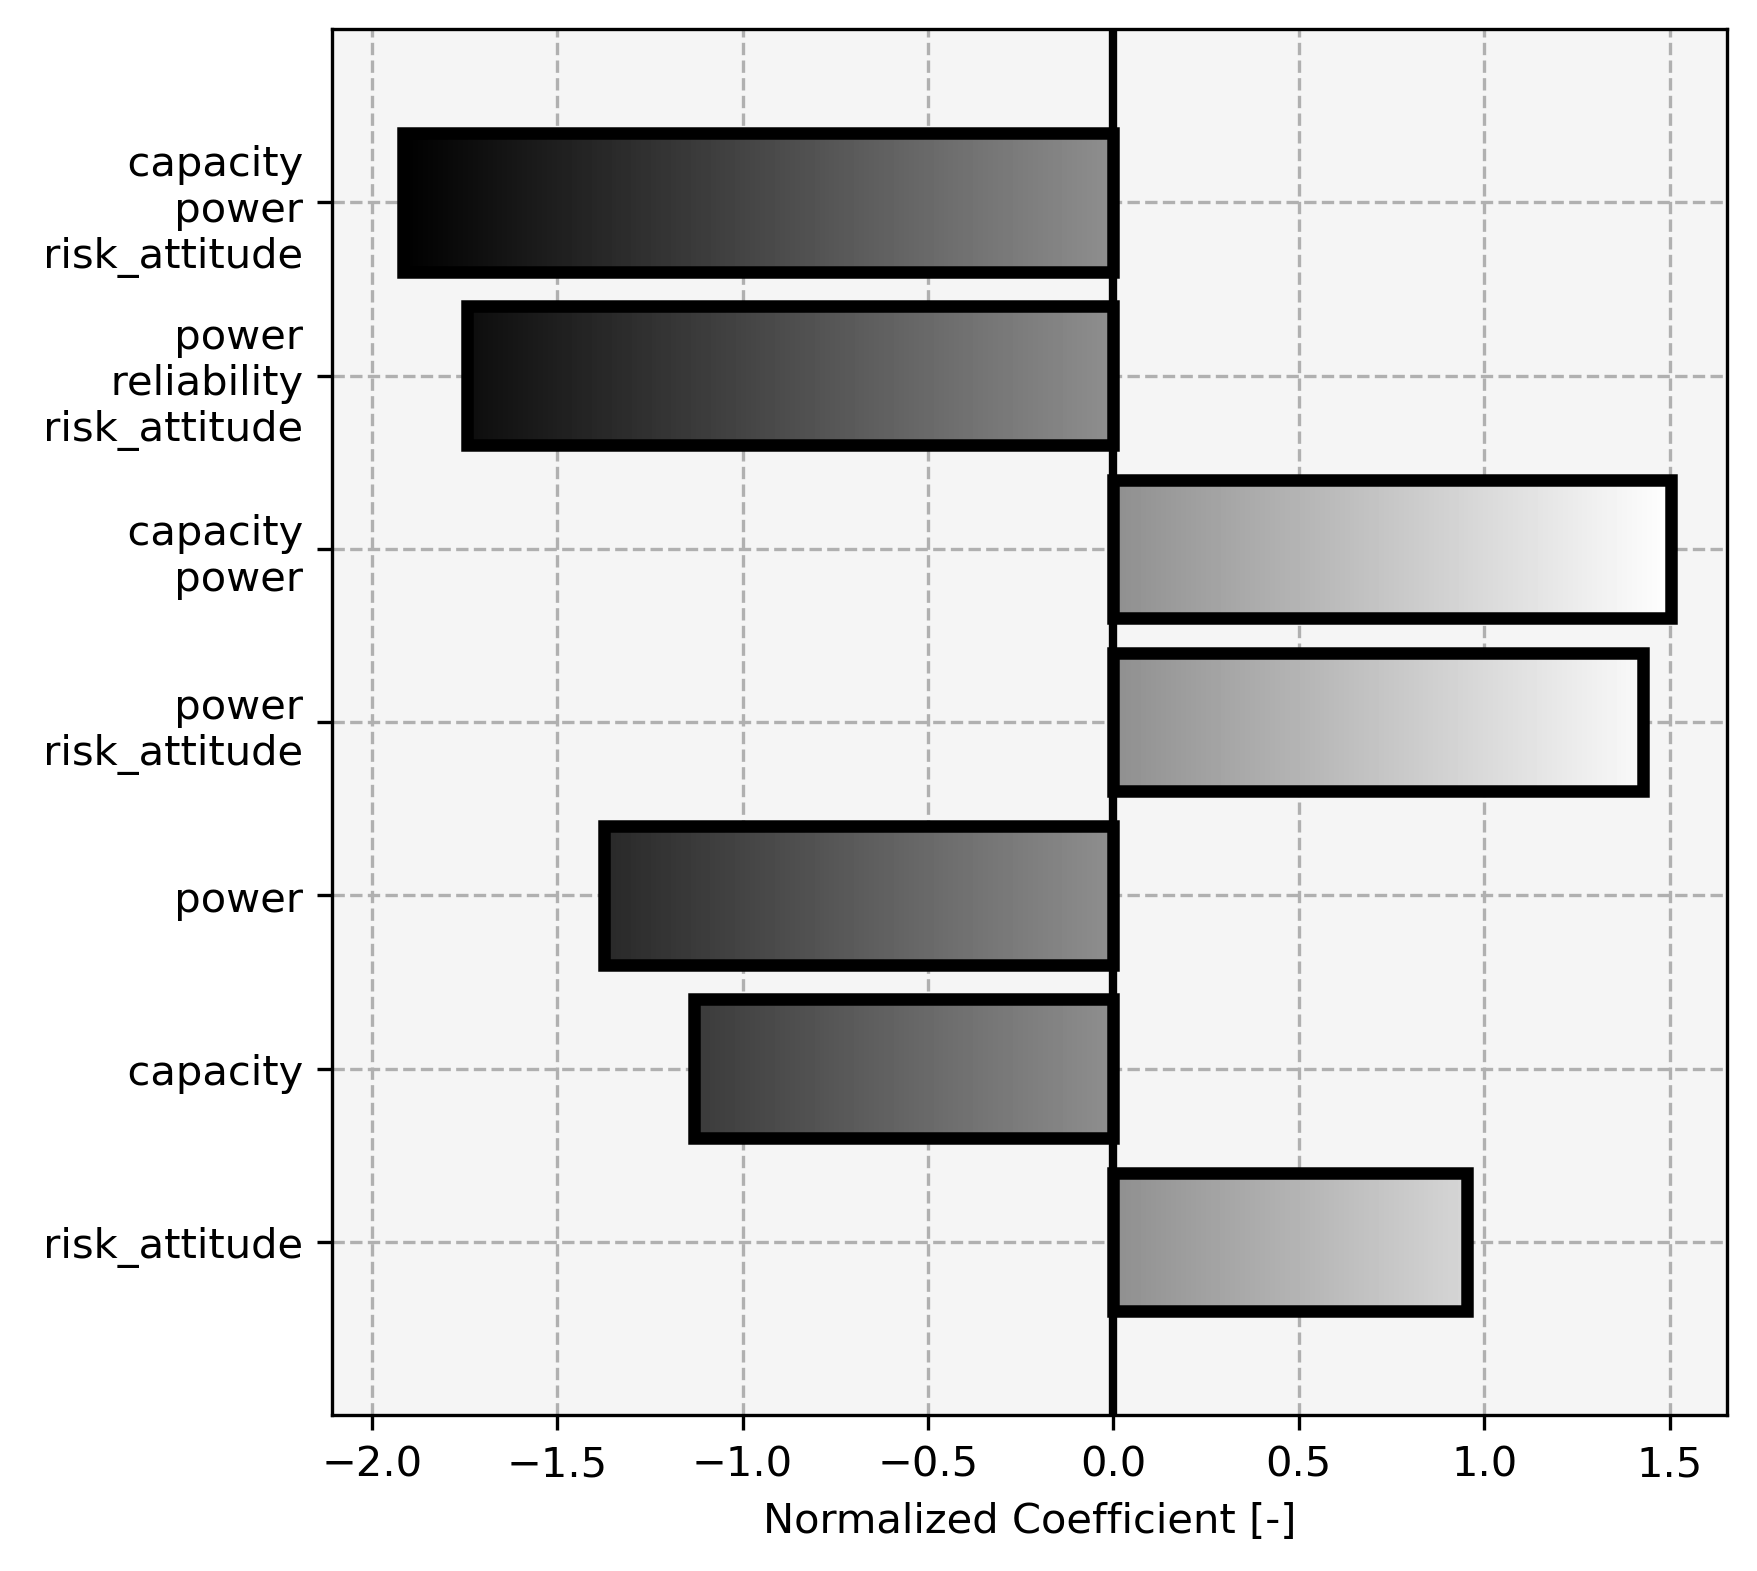
\includegraphics[width = \linewidth]{figs/significant_parameters_2.png}
	\caption{Non-Tesla stations only}
\end{subfigure}

\caption{Coefficients for significant parameters from linear regression}
\label{fig:significant_parameters_0}

\end{figure}

\begin{multicols}{2}

Regardless of \gls{sng}, \gls{ess} capacity and charging power were shown to be significant and important in reducing $Z_R$. The interaction between the two was shown to be subtractive indicating that vehicles with longer ranges benefit less from low recharge times and \textit{vice versa}. Vehicles with high maximum charging speeds can only utilize this advantage at a subset of stations which boast maximum charging speeds equal to or in excess of their own. Vehicles with high ranges have more freedom to choose which stations to utilize on a given route. Past a point, however, these beneficial effects will be saturated. The role of equipment reliability is more complicated. In the model developed herein, poor equipment reliability may cause drivers to opt for paths which appear optimal but are worse in fact due to non-functional equipment. Reliability interacts heavily with risk attitude and in-station redundancy. Where the highly redundant Tesla stations are available the role of reliability in anticipated queuing time is low as, even in the worst case, there is a good chance that the queue will be dissipated. Where these stations are not available, the perceptions of the drivers matter much more in determining expected queuing time. In general, the more and higher quality the stations within a \gls{sng} the less important risk attitude becomes as the fundamental drivers of queuing are lessened. 
	
Some insight into the utility provided by each network can be gained by looking into utilization rates for networks and stations. Ratios of stations utilized at least once to total corridor stations are shown in Figure \ref{fig:utilization_rates}. Most of the utilized chargers belong to the top four networks. Where Tesla stations are available most were utilized at leas once with those not utilized being remote locations. Where Tesla stations are not available, load is shifted towards the other top four networks. This observation indicates that as more vehicles are able to use Tesla stations, traffic will shift towards these stations or other stations which provide similar benefits.

\end{multicols}

\begin{figure}[H]

\begin{subfigure}{\linewidth/3}
	\centering\captionsetup{width = .8\linewidth}
	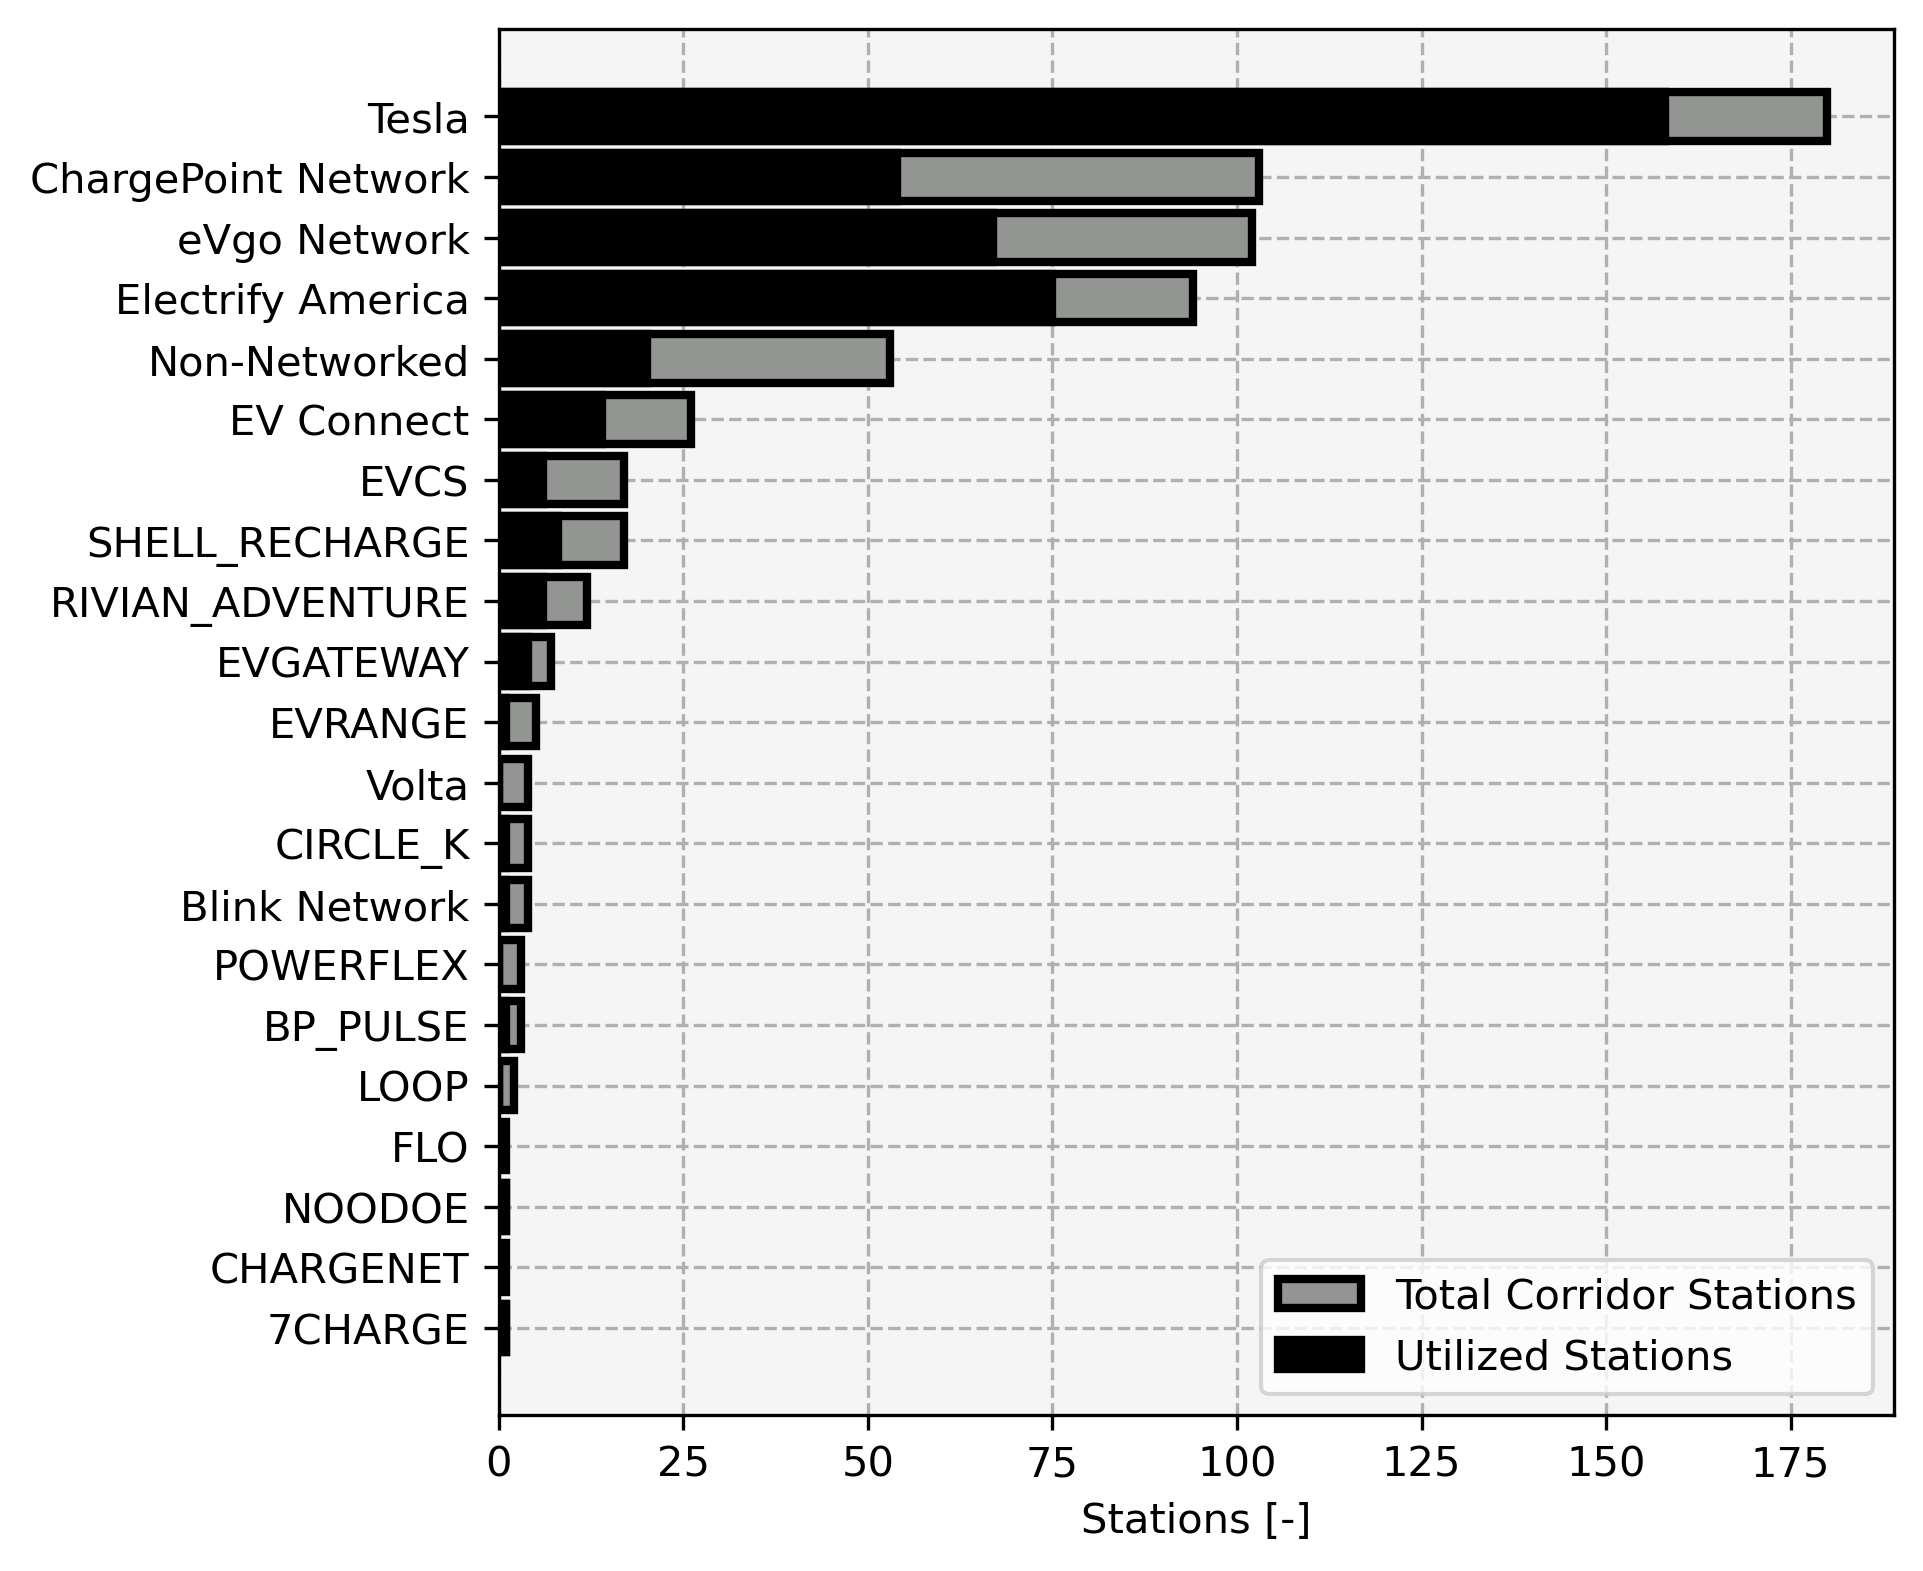
\includegraphics[width = \linewidth]{figs/corridor_station_utilization_0.png}
	\caption{Complete network}
\end{subfigure}%
\begin{subfigure}{\linewidth/3}
	\centering\captionsetup{width = .8\linewidth}
	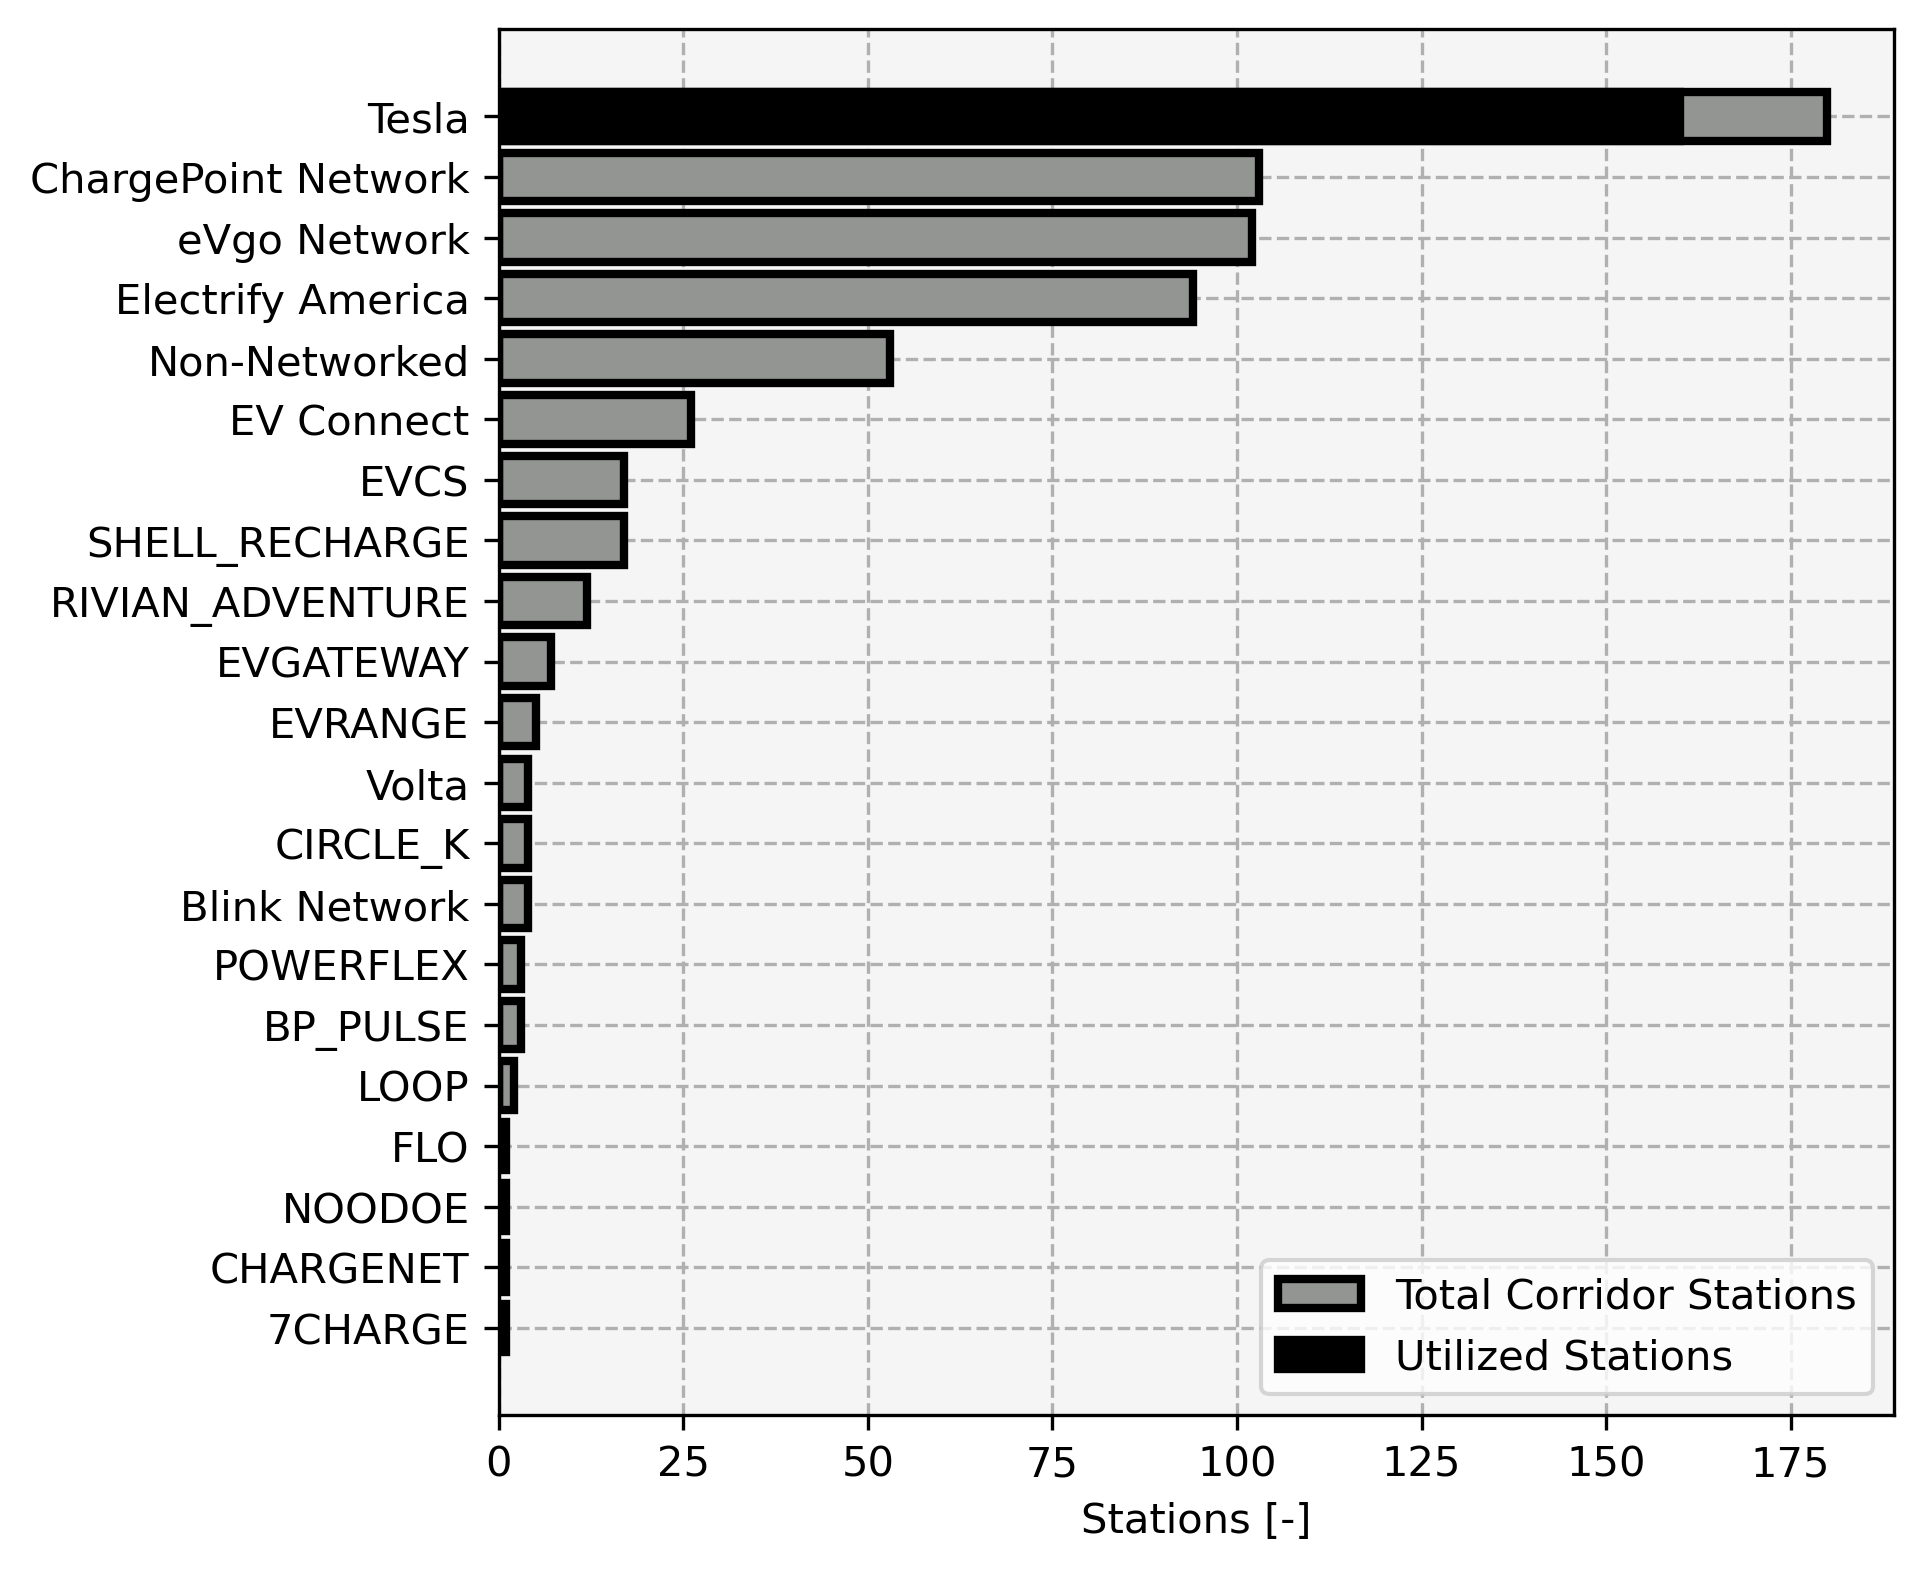
\includegraphics[width = \linewidth]{figs/corridor_station_utilization_1.png}
	\caption{Tesla stations only}
\end{subfigure}%
\begin{subfigure}{\linewidth/3}
	\centering\captionsetup{width = .8\linewidth}
	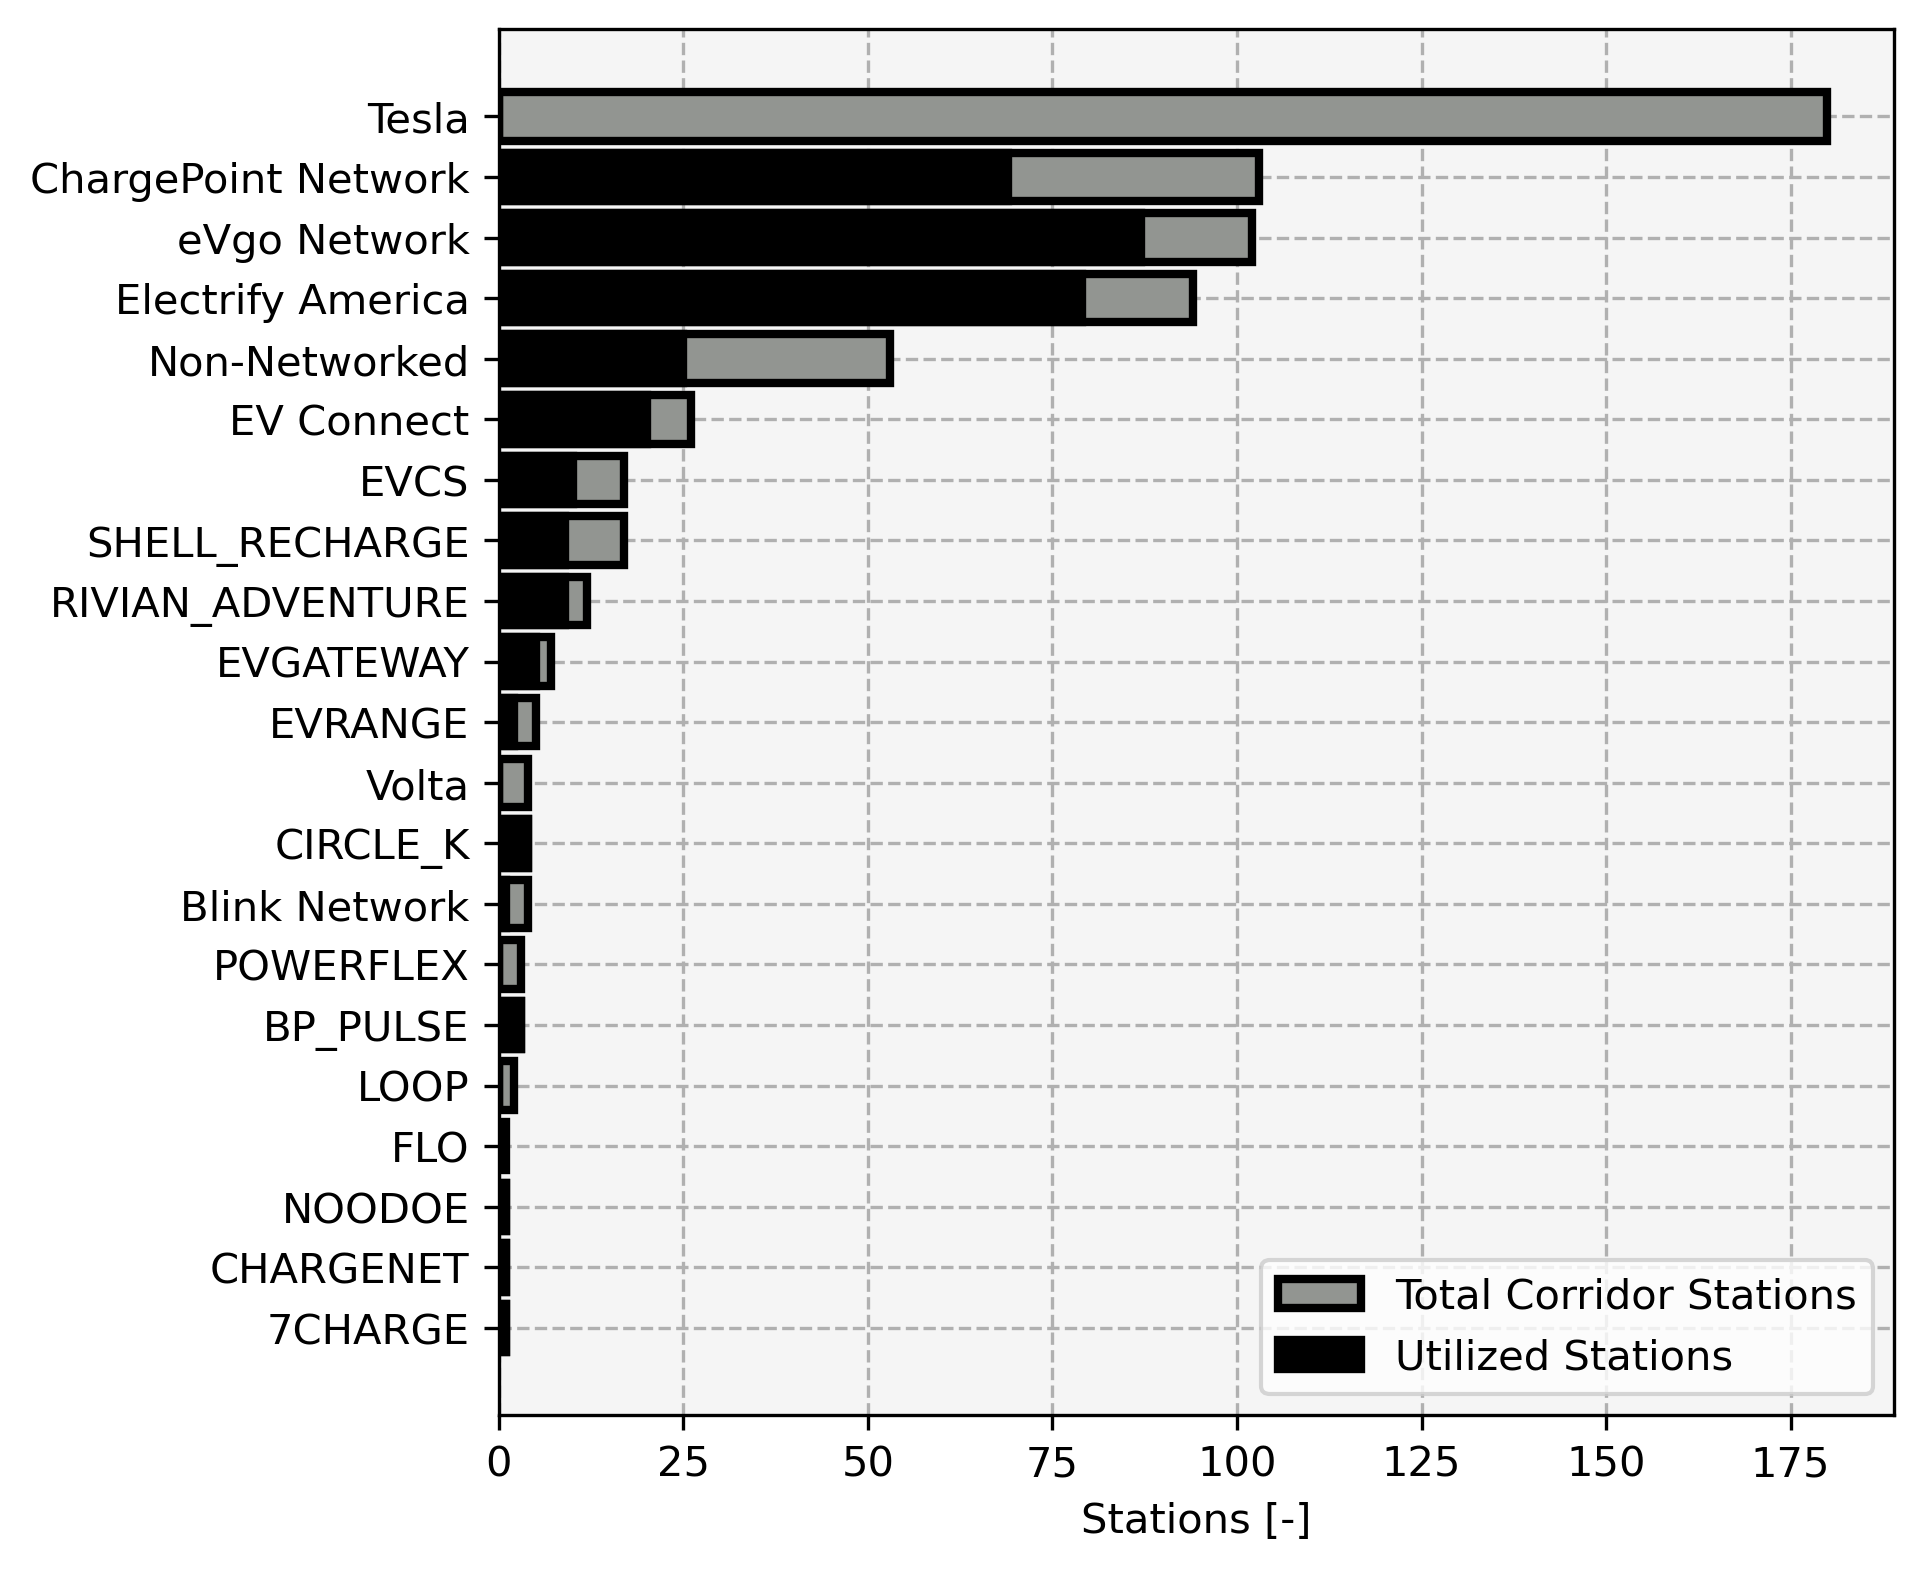
\includegraphics[width = \linewidth]{figs/corridor_station_utilization_2.png}
	\caption{Non-Tesla stations only}
\end{subfigure}

\caption{Ratios of corridor stations utilized at least once to total corridor stations by network for each \gls{sng}.}
\label{fig:utilization_rates}

\end{figure}

\begin{multicols}{2}
	
One important parameter for station utilization is location. Those stations which are most central to the network should see the highest rate of vehicles undertaking long trips passing by. In order to understand the relative value of location as compared to station design, the betweenness centralty for each station, in terms of driving time was computed. Betweenness centrality is the ratio of optimal paths which include a given node to the total number of optimal paths. A second regression analysis was performed on station utilization for the complete \gls{sng}. In this case, the output used was log of utilization (number of times a station appears on an optimal route). Regressors were in-station redundancy and station betweenness centrality using driving time as the cost. Regression results are shown in Tables \ref{tab:utilization_anova} and \ref{tab:utilization_parameters}.

\begin{table}[H]
	\centering
	\caption{Combined Network Linear Regression Analysis ANOVA}
	\label{tab:utilization_anova}
	\begin{tabular}{|C{.25\linewidth}|C{.25\linewidth}|C{.25\linewidth}|C{.25\linewidth}|}
		\hline \rowcolor{lightgray} R & R-Squared & Adjusted R-Squared & Std. Error \\
		\hline 0.614 & 0.377 & 0.371 & 0.005 \\
		\hline \rowcolor{lightgray} Category & Sum of Squares & DOF & Mean Squares \\
		\hline Model & 1135.565 & 3 & 378.522 \\
		\hline Error & 1873.617 & 414 & 4.526 \\
		\hline Total & 3009.182 & 417 & 7.216 \\
		\hline  \rowcolor{lightgray} \multicolumn{2}{|c|}{$F$} &  \multicolumn{2}{c|}{$P(>F)$}  \\
		\hline  \multicolumn{2}{|c|}{83.639} &  \multicolumn{2}{c|}{0.000}  \\
		\hline
	\end{tabular}
\end{table}

\begin{table}[H]
	\centering
	\caption{Combined Network Linear Regression Analysis Coefficients}
	\label{tab:utilization_parameters}
	\begin{tabular}{|C{.5\linewidth}|C{.25\linewidth}|C{.25\linewidth}|}
		\hline \rowcolor{lightgray} Parameter & Coefficient & P-Value \\
		\hline {\small Intercept } & 1.919 & 0.000 \\
		\hline {\small redundancy } & 1.518 & 0.000 \\
		\hline {\small centrality } & 1.181 & 0.330 \\
		\hline {\small redundancy:centrality } & 0.987 & 0.098 \\
		\hline
	\end{tabular}
\end{table}

The two factors can only partially explain the results due to the differences in vehicles and individuals. It is notable that redundancy and interaction terms are significant at $\alpha=0.1$ while centrality, on its own, is not. A possible interpretation is that the redundancy has a more determinant effect and that drivers are sometimes willing to sacrifice route directness in favor of more redundant stations.

\section*{Discussion}

Results of this study suggest that \glspl{bev} drivers experience increased Regional Impedance within California. The expeced difference between a given \gls{icev} and \gls{bev} is roughly 5\%-10\% of total travel time for long trips. A large part of this delta is the unavoidable difference in charging times vs. fueling times. Should \gls{bev} ranges or charging speeds substantially increase the delta will substantially decrease. The rest of the delta is due to the differences between the \glspl{sng} used by \glspl{bev} and \glspl{icev}. the differences within the DC charging \gls{sng} are worth examining in light of continued and future public investment in its build-out.

Because of the structure of the network, Tesla stations are well positioned to absorb traffic should they become fully open to the general light duty \gls{ev} fleet. This may have the result of worsening the user experience at Tesla stations and improving it at other stations until a new equilibrium is reached. The results would also suggest that a second Tesla-style network could enjoy a competitive advantage over the existing non-Tesla networks. It is worth theorizing why such a network has not yet developed. When one single entity has control over all stations in a network and has a captive customer base that network can optimize its expansion. Tesla has, in the past, been able to concentrate chargers to maximize in-station redundancy and minimize between-station redundancy. Simultaneously, Tesla has been able to subsidize overbuilt remote stations with the revenues generated from highly utilized central stations and from car sales. When each network is developed by an independent actor game theoretical considerations come into play. The independent actors must build out their networks under the fear that a competitor could build a competing station near any of their stations at any time. The risk of building station only to lose business to a nearby competitor combined with the opportunity cost of not doing the same results in an inefficient combined network. As Tesla integrates into the wider DC charging network it may begin to behave more like the current non-Tesla companies rather than the other way around. 

What makes the distributed network inefficient are the twin issues of uncertainty and latency. These issues can be mitigated by an integrated status reporting and reservation system. Some information is available to drivers. Crowd sourcing applications such as PlugShare have been available for years allowing drivers to get a better idea of the overall reliability and utilization of stations on the basis of user reviews. Google Maps has recently implemented active plug-level availability monitoring with some, but not all, networks. Finally the private applications of the various networks provide different degrees of information and reservation capability. Future work will investigate the impacts of these systems.

Often, the case for \glspl{bev} is made on an economic basis as \gls{bev} may have lower levelized costs of driving. This study focuses on travel times and routing did not optimize for cost. Partly, this is because at present there is no publicly available data on energy costs at a granular station-level for either gasoline or DC fast charging stations. Nevertheless, some sense of the relative economics of long-trip travel can be attained by examining energy costs per km. Energy costs vary substantially by region in the US with California being the most expensive. Energy costs around the time of writing are shown in Table \ref{tab:energy_costs}.

\begin{table}[H]
	\centering
	\caption{Residential electricity and petroleum average prices USD}
	\label{tab:energy_costs}
	\begin{tabular}{|C{.5\linewidth}|C{.25\linewidth}|C{.25\linewidth}|}
		\hline \rowcolor{lightgray} Source & US & California \\
		\hline Petroleum [gallon] & 3.609 & 5.138 \\
		\hline Residential Electricity [kWh] & 0.1668 & 0.3247 \\
		\hline Transportation Electricity [kWh] & 0.1520 & 0.1191 \\
		\hline DC Fast Charging (Estimated) [kWh] & 0.35 - 0.50 & 0.35 - 0.60 \\
		\hline
	\end{tabular}
\end{table}

Petroleum prices are from AAA \cite{AAA_2024} and electricity prices are from EIA \cite{EIA_2024}. DC fast charging pricing schemes display much heterogeneity and may not be as easily accounted as metered electricity prices. An Ad-Hoc Text Mining study performed on over 90,000 recorded PlugShare events from 2019 and 2021 found the mode of DC fast charging prices to be in the range of 0.3 and 0.4 USD per kWh \cite{Trinko_2021}. Prices did not significantly correlate with local energy prices. In the same time period California residential electricity increased from 0.1995 USD per kWh to 0.2282 USD per kWh and transportation electricity increased from 0.0891 to 0.1179 USD per kWh. By comparison with 2024 electricity prices, one would expect prices in the range of 0.35 and 0.60 USD per kWh for DC fast charging in California and 0.35 to 0.5 in the US, ranges backed by informal reporting \cite{CalTrans_2024, Sowder_2024}. Thus, expected energy costs per highway km traveled can be computed and are shown in Table \ref{tab:expected_energy_costs_per_km}.

\begin{table}[H]
	\centering
	\caption{Expected energy costs per highway km traveled in US cents.}
	\label{tab:expected_energy_costs_per_km}
	\begin{tabular}{|C{\linewidth / 4}|C{\linewidth / 4}|C{\linewidth / 4}|C{\linewidth / 4}|}
		\hline \rowcolor{lightgray} Vehicle & Source & US Price & CA Price \\
		\hline Prius & Petroleum & 4.00 & 5.70 \\
		\hline Golf & Petroleum & 5.47 & 7.78 \\
		\hline Pacifica & Petroleum & 8.97 & 12.77 \\
		\hline \gls{bev} & Residential Electricity & 2.82 & 5.48 \\
		\hline \gls{bev} & DC Fast Charging & 5.91 - 8.44 & 5.91 - 10.13 \\
		\hline
	\end{tabular}
\end{table}

In the US, DC fast charging a \gls{bev} presents no appreciable economic benefit over fueling an efficient \gls{icev}. In much of the US, home-charging a \gls{bev} provides cost savings for daily travel and the initial part of a long trip. This is not the case in California where residential electricity is, on average, nearly twice as expensive as in the US as a whole.

If \glspl{bev} are a worse option than efficient \glspl{icev} for long trips on a time basis and no better on an energy cost basis this will make them less appealing to customers who value the ability to make long road trips. That customers seem to so highly value these uncommon events is a continuing source of frustration for \gls{bev} advocates. Negative perceptions of \gls{bev} long trip utility on consumer stated preference were found to be quite important in the late 2010s \cite{Skippon_2016, Hardman_2016, Franke_2017, Schmalfuss_2017}. In the intervening time period \gls{bev} ranges and maximum charge rates have markedly increased. Nevertheless, negative perceptions related to long trip utility persist for purchasers \cite{Bhat_2022, Paradies_2023, Corradi_2023, Philip_2023} and \gls{bev} range is a significant factor in determining usage share of \glspl{bev} in multi-vehicle household fleets \cite{Chakraborty_2022}. In the same time period, a massive build-out of DC charging infrastructure has taken place yet is not evident that the increased presence of DC charging infrastructure changes perceptions \cite{Hoogland_2023}. It is, sometimes, argued that the time added to a trip due to DC charging is not relevant as breaks are needed regardless. This argument has been used to support the idea that time parity is relatively attainable \cite{Dixon_2020}. While possibly true for a subset of drivers, in order to take advantage of natural breaks to charge a vehicle, the driver must time these breaks to coincide with good charging intervals. The loss of optionality is an inconvenience in this case even if total trip time parity is achieved.

Most travel is not long trip travel. As shown in Figure \ref{fig:utility_factors}, a \gls{bev} with 300 km of range can accomplish 80\% of US daily itineraries on a single charge. Fundamentally, home nd work charging lead to operational costs that are often cheaper and rarely more expensive than petroleum. Similarly, home and work charging can lead to convenience benefits for \glspl{bev} as compared to \glspl{icev} \cite{Rabinowitz_2023} as \glspl{icev} require trips and trip deviations to reach supply stations. In theory, the trade-off of lower cost routine travel for higher cost long-distance travel is one which works in favor of \glspl{bev}. This is the logic which underpins the "charging pyramid" model which places long dwell charging events at its base and corridor DC fast charging events at its peak. This model is also, to some degree, self-reinforcing. If \gls{bev} drivers prefer AC charging, DC charging infrastructure will have limited revenue potential leading to lower network capacity. Lower network capacity, in turn, leads to the perception that the network is inadequate and should be avoided.

The charging pyramid implies a different way of thinking about the role of car travel as a subset an individual's travel needs. Personal travel is inherently multi-modal and, for many \gls{od} arcs and many individuals, the cost differential between different modes is within the threshold of disambiguation. The strengths and weaknesses of \glspl{bev} as compared to \glspl{icev} may shift more short trips away from local transit and towards cars while shifting more long trips away from cars to air travel and inter-city transit. \glspl{bev} will only be one part of future mobility, unable to meet transportation needs or environmental goals on their own. Investments in \gls{bev} corridor infrastructure should be considered alongside investments into other low carbon inter-city transit modes.